%% This template can be used to write a paper for
%% Computer Physics Communications using LaTeX.
%% For authors who want to write a computer program description,
%% an example Program Summary is included that only has to be
%% completed and which will give the correct layout in the
%% preprint and the journal.
%% The `elsarticle' style is used and more information on this style
%% can be found at 
%% http://www.elsevier.com/wps/find/authorsview.authors/elsarticle.
%%
%%
%% \documentclass[preprint,12pt]{elsarticle}

%% Use the option review to obtain double line spacing
%% \documentclass[preprint,review,12pt]{elsarticle}

%% Use the options 1p,twocolumn; 3p; 3p,twocolumn; 5p; or 5p,twocolumn
%% for a journal layout:
\documentclass[final,1p,times]{elsarticle}
%% \documentclass[final,1p,times,twocolumn]{elsarticle}
%% \documentclass[final,3p,times]{elsarticle}
%% \documentclass[final,3p,times,twocolumn]{elsarticle}
%% \documentclass[final,5p,times]{elsarticle}
%% \documentclass[final,5p,times,twocolumn]{elsarticle}

%% if you use PostScript figures in your article
%% use the graphics package for simple commands
%% \usepackage{graphics}
%% or use the graphicx package for more complicated commands
%% \usepackage{graphicx}
%% or use the epsfig package if you prefer to use the old commands
%% \usepackage{epsfig}

%% The amssymb package provides various useful mathematical symbols
\usepackage{amssymb}
\usepackage{amsmath}    % need for subequations
\usepackage{graphicx}   % need for figures
\usepackage{verbatim}   % useful for program listings
\usepackage{color}      % use if color is used in text
\usepackage{subfigure}  % use for side-by-side figures
\usepackage{hyperref}   % use for hypertext links, including those to external

%% The amsthm package provides extended theorem environments
%% \usepackage{amsthm}

%% The lineno packages adds line numbers. Start line numbering with
%% \begin{linenumbers}, end it with \end{linenumbers}. Or switch it on
%% for the whole article with \linenumbers after \end{frontmatter}.
%% \usepackage{lineno}

%% natbib.sty is loaded by default. However, natbib options can be
%% provided with \biboptions{...} command. Following options are
%% valid:

%%   round  -  round parentheses are used (default)
%%   square -  square brackets are used   [option]
%%   curly  -  curly braces are used      {option}
%%   angle  -  angle brackets are used    <option>
%%   semicolon  -  multiple citations separated by semi-colon
%%   colon  - same as semicolon, an earlier confusion
%%   comma  -  separated by comma
%%   numbers-  selects numerical citations
%%   super  -  numerical citations as superscripts
%%   sort   -  sorts multiple citations according to order in ref. list
%%   sort&compress   -  like sort, but also compresses numerical citations
%%   compress - compresses without sorting
%%
%% \biboptions{comma,round}

% \biboptions{}

%% This list environment is used for the references in the
%% Program Summary
%%
\newcounter{bla}
\newenvironment{refnummer}{%
\list{[\arabic{bla}]}%
{\usecounter{bla}%
 \setlength{\itemindent}{0pt}%
 \setlength{\topsep}{0pt}%
 \setlength{\itemsep}{0pt}%
 \setlength{\labelsep}{2pt}%
 \setlength{\listparindent}{0pt}%
 \settowidth{\labelwidth}{[9]}%
 \setlength{\leftmargin}{\labelwidth}%
 \addtolength{\leftmargin}{\labelsep}%
 \setlength{\rightmargin}{0pt}}}
 {\endlist}

\journal{Computer Physics Communications}

\begin{document}

\begin{frontmatter}

%% Title, authors and addresses

%% use the tnoteref command within \title for footnotes;
%% use the tnotetext command for the associated footnote;
%% use the fnref command within \author or \address for footnotes;
%% use the fntext command for the associated footnote;
%% use the corref command within \author for corresponding author footnotes;
%% use the cortext command for the associated footnote;
%% use the ead command for the email address,
%% and the form \ead[url] for the home page:
%%
%% \title{Title\tnoteref{label1}}
%% \tnotetext[label1]{}
%% \author{Name\corref{cor1}\fnref{label2}}
%% \ead{email address}
%% \ead[url]{home page}
%% \fntext[label2]{}
%% \cortext[cor1]{}
%% \address{Address\fnref{label3}}
%% \fntext[label3]{}

\title{TensorAlloy: an automatic atomistic neural network program for alloys}

%% use optional labels to link authors explicitly to addresses:
%% \author[label1,label2]{<author name>}
%% \address[label1]{<address>}
%% \address[label2]{<address>}

\author[a]{Xin Chen}
\author[a]{Xing-Yu Gao}
\author[b]{Ya-Fan Zhao}
\author[b]{De-Ye Lin\corref{author}}
\author[a]{Wei-Dong Chu}
\author[a,b]{Hai-Feng Song\corref{author}}

\cortext[author] {Corresponding author.
\\\textit{E-mail address:} lindeye0716@163.com}
\address[a]{Institute of Applied Physics and Computational Mathematics, 
Beijing 100088, China}
\address[b]{CAEP Software Center for High Performance Numerical Simulation, 
Beijing 100088, China}

\begin{abstract}
Atomistic modeling is important for studying physical and chemical properties of
materials. Recently, machine learning interaction potentials have gained much 
more attentions as they can provide density functional theory level predictions 
within negligible time. The symmetry function descriptor based 
atomistic neural network is the most widely used model for modeling alloys. 
To precisely describe complex potential energy surfaces, integrating advanced 
metrics, such as force or virial stress, into training can be of great help.  
In this work, we propose a virtual-atom approach to model the total energy of 
symmetry function descriptors based atomistic neural network. Our approach 
creates the computation graph directly from atomic positions. Thus, the 
derivations of forces and virial can be handled by TensorFlow automatically and 
efficiently. The virtual atom approach with AutoGrad within TensorFlow allows 
for efficient training to not just energies and forces, but also virial stress. 
This new approach is implemented in our open-source program TensorAlloy, which 
supports constructing machine learning interaction potentials for both 
\textit{molecules} and \textit{solids}. The QM7 and SNAP/Ni-Mo datasets are used 
to demostrate the performances of our program.
\end{abstract}

\begin{keyword}
%% keywords here, in the form: keyword \sep keyword
Machine Learning; Alloy; Materials Modeling; Computational Physics; 
Neural Network

\end{keyword}

\end{frontmatter}

%%
%% Start line numbering here if you want
%%
% \linenumbers

% Computer program descriptions should contain the following
% PROGRAM SUMMARY.

{\bf PROGRAM SUMMARY} \\
\begin{small}
\noindent
{\em Program Title: TensorAlloy} \\
{\em Licensing provisions(please choose one): LGPL}           \\
{\em Programming language: Python 3.7}                        \\
{\em Supplementary material:}                                 \\
{\em Journal reference of previous version:}                  \\
{\em Does the new version supersede the previous version?:}   \\
{\em Reasons for the new version:} \\
{\em Summary of revisions:}*\\
{\em Nature of problem:} \\
  Modeling interatomic interactions with the symmetry function descriptor based
  atomistic neural networks.
{\em Solution method:} \\
  The TensorAlloy program is built upon TensorFlow and the virtual-atom 
  approach. TensorAlloy can build direct computation graph from atomic positions 
  to total energy. Atomic forces and virial stress tensors are handled by 
  TensorFlow automatically and efficiently. \\
{\em Additional comments including Restrictions and Unusual features}\\
  This program needs TensorFlow 1.13.*. Neither newer or older TensorFlow is 
  supported. \\
\end{small}

% % % % % % % % % % % % % % % % % % % % % % % % % % % % % % % % % % % % % % % %
% 
% Section 1. Introduction
%
% % % % % % % % % % % % % % % % % % % % % % % % % % % % % % % % % % % % % % % %
\section{Introduction}

Atomistic simulations (\textit{ab initio} calculation, classic molecular 
dynamics simulation (MD), etc) are powerful tools for studying physical and 
chemical properties of materials. To obtain reliable simulation results, 
atomistic interactions must be properly described. The very accurate 
\textit{ab initio} and quantum chemical methods have gain significant 
improvements over the past decades but their applicabilities are restricted by 
computation expenses. Physical model based empirical potentials, such as the 
embedded-atom method\cite{eam-1,eam-2,eam-3,eam-4,eam-5} or its variants (
modified embedded-atom method\cite{eam-5,meam-1,meam-2,meam-3}, 
angular-dependent interaction potential\cite{adp-1,adp-2,adp-3}, etc), are much 
more popular for long-time simulation because of their reasonable accuraty and 
acceptable costs. 
However, designing empirical potentials and optimizing parameters for 
alloys are still challenging tasks\cite{eam-5, adp-2, SNAP_2018}. 

In the past few years, machine learning (ML) has become one of the most 
influential topic in almost all fields of science. A lot of effort has been made 
by various physicists to explore the possiblity of using ML models \textemdash 
instead of traditional empirical potentials \textemdash to describe atomistic 
interactions during MD simulations\cite{kCON,SchNet,DTNN,SNAP_2018,SNAP_Mo_2017,
ANI,TensorMol}. ML potentials are much easier to design and 
optimize. With sufficient training data, ML models can achieve similar or even 
better performances compared with density functional theory.
The symmetry function based atomistic neural network (ANN) model, first proposed 
by Parinello and Behler in 2007\cite{Behler,Behler2,Behler3,Behler4,Behler1}, 
is still the most widely used method for \textit{solids} and its effectness and 
accuracy has been proven by several 
works\cite{Behler-solids-lzp-1,Behler-alloy-1,Behler-alloy-2, Behler-alloy-3}.
Until now, various ML implementations\cite{AMP,ANI,TensorMol} have been 
published by researchers. The Amp\cite{AMP} package, developed by Peterson's 
group, is the first open-source framework that implements the symmetry function 
descriptor. Amp can be used to learn interaction potentials for both 
\textit{molecules} and \textit{solids} and it has successfully powered quite a 
few researches since 2016\cite{Amp-works-hammer,amp-work-1}. 
TensorMol\cite{TensorMol} and its sucessor TorchANI\cite{ANI} are also symmetry 
function based ANN programs but they mainly focus on \textit{molecules}. 

In order to precisely model atomistic interactions, both total energy and atomic 
forces are necessary. For \textit{solids}, the virial stress tensor is also an
essential metric. However, integrating force and stress into the loss function 
is not an easy task. The machine learning approaches favor vectorizable 
operations but the calculations of atomic descriptors are typically complicated 
so that many traditional ML packages (Amp, kCON, etc) choose to pre-compute 
descriptors and only build computation graph from descriptors to total energy. 
This traditional approach can significantly reduce technical difficulty and 
works very well if only total energy is considered in the loss function. But to 
fit atomic forces, numerous codes must be written manually, such as the 
derivation of descriptors with respect to positions. Although the derivation is 
theoretically clear, the implementation is challenging and the efficiency can 
not be guaranteed.

Recently, machine learning platforms (TensorFlow\cite{tensorflow}, 
PyTorch\cite{pytorch}, MXNet\cite{MXNet}, etc) have gain significant 
developments. These modern machine learning frameworks can fully take advantage 
of GPUs for acceleration. The automatic differentiation capability brings a new 
route for devloping ML models capable of predicting energy, force and stress as 
we may 'let' ML platforms to handle the calculations of force and stress because 
these metrics can be derived from positions and total energy directly. To 
achieve this, a direct computation graph from positions to total energy must be
built. Thus, the problem becomes: how to design such route?

In this work, we propose a new TensorFlow-dependent apporach (the virtual atom 
approach, VAP) to model the total energy expression of the symmetry function 
descriptor based neural network. 
Our apporach can move the entry of the computation graph from atomic descriptors 
back to the raw atomic positions. Thus, calculating the derivatives of total 
energy with respect to atomic positons (force) or lattice tensor (virial) can be 
handled by TensorFlow directly and automatically. Hence, the technical barrier 
of training ANNs with atomic forces and (especially) virial stress becomes 
completely neglectable.

This paper is organized as follows. Section \ref{section:theory} introduces the 
theory of the symmetry function descriptor and the ANN framework. Section 
\ref{section:method} describes the virtual atom approach and the modified ANN 
model used by TensorAlloy. Section \ref{section:discussions} demostrates 
the performances of TensorAlloy on two public datasets. The appendix 
\ref{section:appendix} gives derivation and implementation details of key 
routines of VAP. 

% % % % % % % % % % % % % % % % % % % % % % % % % % % % % % % % % % % % % % % %
% 
% New Commands
%
% % % % % % % % % % % % % % % % % % % % % % % % % % % % % % % % % % % % % % % %

\newcommand{\rijn}{r_{ij\mathbf{n}}}
\newcommand{\rijna}{r_{ij\mathbf{n_1}}}
\newcommand{\rikna}{r_{ik\mathbf{n_2}}}
\newcommand{\rjkna}{r_{jk\mathbf{n_3}}}

\newcommand{\nmax}{
    N_{\mathrm{Ni}}^{\mathrm{max}}+N_{\mathrm{Mo}}^{\mathrm{max}}
}
\newcommand{\nijmax}{N_{ij}^{\mathrm{max}}}
\newcommand{\nijkmax}{N_{ijk}^{\mathrm{max}}}
\newcommand{\nelmax}{N^{\mathrm{max}}_{\mathrm{el}}}
\newcommand{\nel}{N_{\mathrm{element}}}
\newcommand{\nvap}{N^{\mathrm{vap}}}
\newcommand{\nnimax}{N^{\mathrm{max}}_{\mathrm{Ni}}}
\newcommand{\nmomax}{N^{\mathrm{max}}_{\mathrm{Mo}}}

% % % % % % % % % % % % % % % % % % % % % % % % % % % % % % % % % % % % % % % %
% 
% Section 2. Theory
%
% % % % % % % % % % % % % % % % % % % % % % % % % % % % % % % % % % % % % % % %
\section{Theory}
\label{section:theory}

In the atomistic neural network (\textbf{ANN}) framework, the total energy, 
$E^{total}$, of a structure with $N$ atoms, can be expressed as the sum of all 
atomic energies:
\begin{equation}
\label{eq:general_e_total}
E^{total} = \sum_{i}^{N}{E_i}
\end{equation}
where $E_{i}$, the energy of atom \textit{i}, is the output of the neural 
network $\mathbf{NN}_{el}$ for element $el$:
\begin{equation}
E_i = \mathbf{NN}_{el}\left( \mathbf{G}_i \right)
\end{equation} 
Here $\mathbf{G}_i$ is a vector representing atomic descriptors of atom $i$. 
$\mathbf{G}_i$ typically only depends on local environment of atom $i$, i.e.  
its neighbors:
\begin{equation}
\mathbf{G}_i = F_G(\left\{ \rijn, |\rijn| < r_c\right\} )
\end{equation}
where $F_G$ is a specifc feature function, $r_c$ is the cutoff radius and 
$\rijn$ is the interatomic distance considering the periodic boundary 
conditions: 
\begin{equation}
    \label{eq:rijn}
    \rijn = \Vert \mathbf{r}_i^{(0)} - \mathbf{r}_j^{(0)} + 
    \mathbf{n}^T \mathbf{h} \Vert
\end{equation}
where $\mathbf{r}_i^{(0)}$ and $\mathbf{r}_j^{(0)}$ denote positions of atoms 
$i$ and $j$ in the primitive cell, $\mathbf{n}$ is a column vector specifying 
the cell shifts along $(X,Y,Z)$ directions
\begin{equation}
    \label{eq:ij_shift}
    \mathbf{n} = \begin{pmatrix}
        n_x \\
        n_y \\
        n_z
    \end{pmatrix}
\end{equation}
and $\mathbf{h}$ is the \textbf{row-major} $3 \times 3$ lattice tensor:
\begin{equation}
    \label{eq:lattice}
    \mathbf{h} = \begin{pmatrix}
        h_{xx} & h_{xy} & h_{xz} \\
        h_{yx} & h_{yy} & h_{yz} \\
        h_{zx} & h_{zy} & h_{zz} \\
    \end{pmatrix}
\end{equation}

There are many choices of $F_G$. The symmetry function descriptor, proposed 
by Parinello and Behler in 2007\cite{Behler}, is currently the most widely used 
atomic descriptor. The symmetry function descriptor consists of two types of 
functions: the radial symmetry function $\mathbf{G}^{(2)}$ and the angular 
symmetry function $\mathbf{G}^{(4)}$:
\begin{align}
\label{eq:G2}
\mathbf{G}^{(2)}_i(\eta, \omega) = & \sum_{j \neq i}{
    \sum_{\mathbf{n}}{g_2 (\eta, i, j, \omega)}
} \\
\label{eq:G4}
\mathbf{G}^{(4)}_i(\beta, \gamma, \zeta) 
= & 2^{1-\zeta}\sum_{j, k\neq j, k\neq i}{
    \sum_{\mathbf{n}_1}{\sum_{\mathbf{n}_2}{\sum_{\mathbf{n}_3}{
        g_4(\beta, \gamma, \zeta, 
          i, j, k, 
          \mathbf{n}_1, \mathbf{n}_2, \mathbf{n}_3)
    }}}
} \\
\label{eq:g2}
g_2(\eta, i, j, \omega) = 
& \exp\left\{-\frac{\eta(\rijn - \omega)^2}{r_c^2} \right\} \cdot f_c(\rijn) \\
\label{eq:g4}
g_4(
    \beta, \gamma, \zeta, 
    i, j, k, 
    \mathbf{n}_1, \mathbf{n}_2, \mathbf{n}_3) = & 
\left( 1 + \gamma\cos\theta \right)^\zeta 
    \exp \left\{ -\frac{\beta(\rijna^2 + \rikna^2 + \rjkna^2)}{r_c^2} \right\}
\nonumber \\
& \times f_c(\rijna)f_c(\rikna)f_c(\rjkna)
\end{align}
where $\eta$, $\omega$, $\beta$, $\gamma$ and $\zeta$ are empirically chosen 
parameters, $f_c(r)$ is a cutoff (damping) function and its original form is:
\begin{equation}
\label{eq:fc_origin}
f_c(r) =
    \begin{cases}
    0 & \text{$r > r_c$} \\
    \frac{1}{2} + \frac{1}{2}\cos\left(r / r_c \cdot \pi \right) & 
    \text{$r \leq r_c$}
    \end{cases}
\end{equation}
and $r_c$ is the cutoff radius. Equation \eqref{eq:fc_origin} can be further 
transformed to a vectorized expression:
\begin{equation}
\label{eq:fc}
f_c(r) = \frac{1}{2}\left( 
    1 + \cos\left[ \min(\frac{r}{r_c}, 1) \pi \right] 
\right)
\end{equation} 
and $\cos\theta$ also has a vectorized form:
\begin{equation}
\cos\theta = \frac{\rijna^2 + \rikna^2 - \rjkna^2}{2 \rijna \cdot \rikna}
\end{equation}
The summations in Equation \ref{eq:G2} and \ref{eq:G4} should go over all 
neighbors within $r_c$. For an atom $i$, $\mathbf{G}_i$ is a vector. For the 
entire structure, its overall $\mathbf{G}$ is a matrix with row $i$ represents 
the atomic descriptors of atom $i$ and column $j$ corresponds to a specifc 
$(\eta, \omega)$ pair or $(\beta, \gamma, \zeta)$ combination.

Analytical atomic forces can be obtained directly by computing the first-order 
derivative of $E^{total}$ with respect to $\mathbf{r}_{a}^{(0)}$ where $a$ is an 
index:
\begin{equation}
\label{eq:dEdr}
f_a = -\frac{\partial E^{total}}{\partial \mathbf{r}_a^{(0)}}
\end{equation}
According to the chain rule, we can expand Equation \ref{eq:dEdr}:
\begin{align}
\frac{\partial E^{total}}{\partial \mathbf{r}_a^{(0)}} = & \sum_{i}^{N}{
    \frac{
        \partial\mathbf{NN}_{el}(\mathbf{G}_i)}{
        \partial \mathbf{r}_a^{(0)}}} \nonumber \\
= & \sum_{i}^{N}{\sum_{l}^{N_G}{
    \frac{\partial \mathbf{NN}_{el}(\mathbf{G}_i)}{\partial G_{il}}
    \cdot
    \frac{\partial G_{il}}{\partial \mathbf{r}_{a}^{(0)}}
}}
\end{align}
and 
\begin{align}
\frac{\partial G_{il}^{(2)}}{\partial \mathbf{r}_{a}^{(0)}} = & \sum_{j \neq i}{
    \sum_{\mathbf{n}}{
        \frac{\partial g_2}{\partial \rijn}
        \cdot
        \frac{\partial \rijn}{\partial r_k^{0}}
    }
} \\
\frac{\partial G_{il}^{(4)}}{\partial \mathbf{r}_{a}^{(0)}} = &
2^{1 - \zeta}\sum_{j, k \neq j, k \neq i}{
    \sum_{\mathbf{n}_1}{\sum_{\mathbf{n}_2}{\sum_{\mathbf{n}_3}{
        \left(
            \frac{\partial g_4}{\partial \rijna}
            \frac{\partial \rijna}{\partial \mathbf{r}_{a}^{(0)}} + 
            \frac{\partial g_4}{\partial \rikna}
            \frac{\partial \rikna}{\partial \mathbf{r}_{a}^{(0)}} + 
            \frac{\partial g_4}{\partial \rjkna}
            \frac{\partial \rjkna}{\partial \mathbf{r}_{a}^{(0)}}
        \right)
    }}}
}
\end{align}

The derivations are theoretically straightforward but their implementations are 
challenging \cite{AMP}. Later we will provide an automatic approach to address 
this problem.

The $3 \times 3$ virial tensor $\epsilon$ is an important metric to 
describe solids under deformation or external pressure. For arbitrary many-body 
interaction potentials, $\epsilon$ can be calculated with the following equation
\cite{lammps_stress}:
\begin{equation}
\label{eq:stress_lammps}
\epsilon = \left(-\sum_{i=1}^{N}{\mathbf{r}_i^{(0)} \otimes f_i} - 
\sum_{\mathbf{n}}{\mathbf{h}^T\mathbf{n}} \otimes 
\sum_{i=1}^{N}{F^{\prime}_{i\mathbf{n}}}
\right)^T
\end{equation}
where $\otimes$ indicates tensor product, $f_i$ is the total 
force acting on atom $i$ and $F^{\prime}_{i\mathbf{n}}$ is the partial force. 
Until now, most machine learning force-field models focus on fitting total 
energy and atomic forces, very few of them\cite{DeePMD,DeePMD_rl,DeePMD_kit} had 
attempted to include stress in their loss functions. 
The current expression of Equation \ref{eq:stress_lammps} is not very compatible 
with NN or other ML potentials since the partial forces are difficult to compute 
with vectorized operations. However, we find an "equivalent" form 
of Equation \ref{eq:stress_lammps}:
\begin{equation}
\label{eq:stress}
\epsilon = -F^{T} R + 
\left(\frac{\partial E^{total}}{\partial \mathbf{h}}\right)^T \mathbf{h}
\end{equation}
where $R$ is the $N \times 3$ positions matrix and $F$ is the 
corresponding total forces matrix. This new form can be easily implemented 
within TensorFlow. The detailed derivation is given in the appendix(A).

% % % % % % % % % % % % % % % % % % % % % % % % % % % % % % % % % % % % % % % %
% 
% Section 3. Method
%
% % % % % % % % % % % % % % % % % % % % % % % % % % % % % % % % % % % % % % % %
\section{Method}
\label{section:method}

In this section we will describe the architecture of TensorAlloy and the core 
algorithm: the virtual atom approach (VAP). The most noticable feature of the 
TensorAlloy program is that the calculation of symmetry function descriptors is 
automatically handled by the \textbf{AutoGrad}\cite{tensorflow} routine of 
TensorFlow because we successfully find a route (VAP) to build the direct 
computation graph from atomic positions to total energy.

The Ni-Mo binary alloy system will be used as the example to show our 
algorithms. The original dataset (SNAP) is published by Shyue Ping 
Ong\cite{SNAP_2018}. 
For simplicity, only radial symmetry function related algorithms are 
visualized in the figures. Python3.7 implementations of key algorithms and 
functions are given in the appendix. 

% % % % % % % % % % % % % % % % % % % % % % % % % % % % % % % % % % % % % % % %
% 
% Section 3.A
%
% % % % % % % % % % % % % % % % % % % % % % % % % % % % % % % % % % % % % % % %
\subsection{Overview}
\label{section:overview}

Fig \ref{fig:program_design} shows the overview of TensorAlloy and the 
virtual-atom approach.
TensorAlloy has two phases: the training phase \textbf{(1)} and the prediction 
phase \textbf{(2)}. These two phases share many common requirements, but they 
also have their own concerns.

For the training phase, in order to make TensorAlloy a general-purpose and
efficient machine learning potential training program, there are some key 
technical requirements:
\begin{itemize}
    
    \item[1.] 
    Stoichiometry-free: the training dataset should not have any stoichiometry 
    restriction. Any type of \textit{solid} or \textit{molecule} is acceptable. 
    A universal approach of expressing different structures in a single 
    reference system may be necessary.
    
    \item[2.] 
    Mini-batch training: mini-batch based stochastic training is 
    currently the most efficient way to train neural networks on large datasets.
    However, batch training requires \textit{vectorized} and \textit{aligned} 
    expressions. Here \textit{aligned} means feature arrays of structures of 
    different stoichiometries share the same shape. 
    
    \item[3.] 
    Cache: some intermediate arrays may be pre-computed and stored in cache 
    files. During training, these values can be loaded from cache directly, thus 
    saving significantly amount of resources.

\end{itemize}

In the prediction phase, the situation is a bit different. The stoichiometry of 
the target structure or molecule may not be included in the training dataset and 
it can vary significantly. TensorAlloy must be capable of handling such 
(extreme) situations. For example, the trained Ni-Mo shall be applicable to any 
any $\mathrm{Ni}_{x}\mathrm{Mo}_{y}$ structure while $x$ and $y$ can be 
either as large as 100000 or as small as 0. 

Besides, we also want our TensorAlloy program have an \textit{independent} and
\textit{user-friendly} prediction phase. Users can just focus on the integration 
of machine learning potentials with their own researches.

VAP plays a central role in handling all the technical challenge as it 
\textbf{\textit{provides a way to describe structures of various sizes and 
stoichiometries in unified and vectorized forms}}. 
In the following sections, we will gradually discuss the details of this 
approach.

% % % % % % % % % % % % % % % % % % % % % % % % % % % % % % % % % % % % % % % %
% 
% Fig.1
%
% % % % % % % % % % % % % % % % % % % % % % % % % % % % % % % % % % % % % % % %
\begin{figure}[h!]
\centering
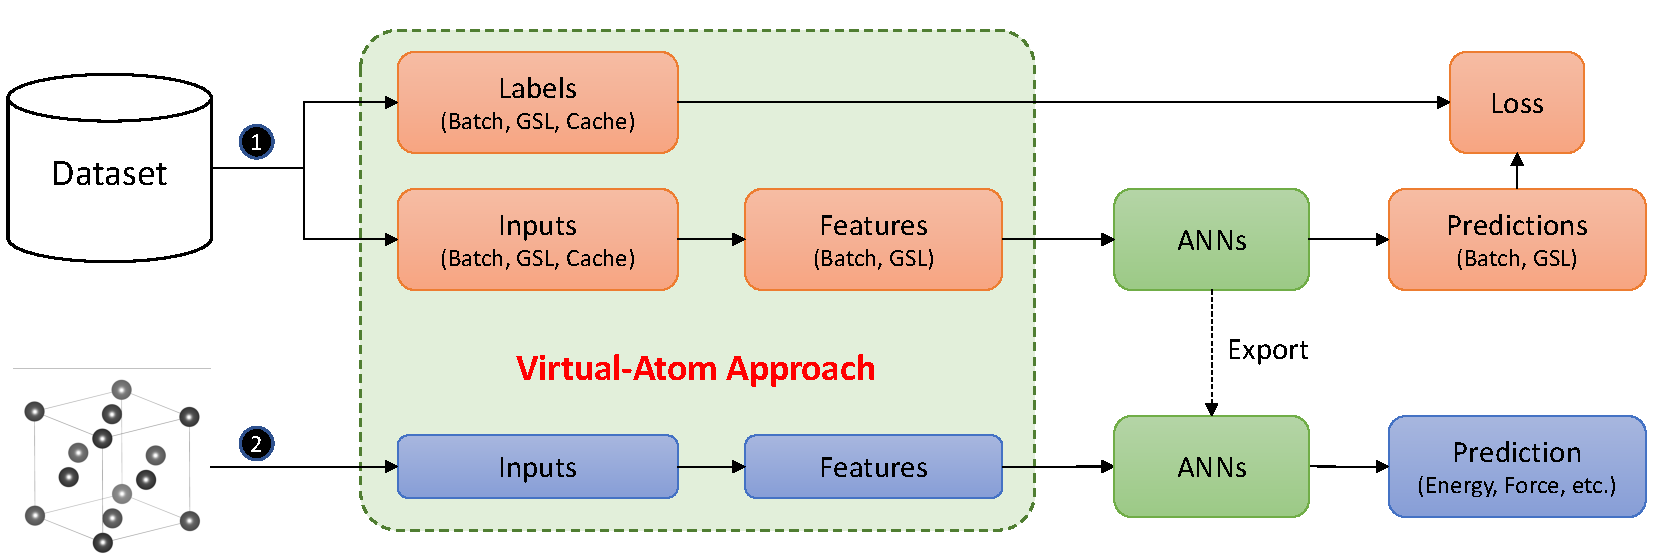
\includegraphics[scale=0.55]{figures/Fig1.pdf}
\caption{\label{fig:program_design} The general design of TensorAlloy. 
\textbf{(1)} demonstrates the training phase while \textbf{(2)} represents the 
prediction phase.
}
\end{figure}

% % % % % % % % % % % % % % % % % % % % % % % % % % % % % % % % % % % % % % % %
% 
% Section 3.B
%
% % % % % % % % % % % % % % % % % % % % % % % % % % % % % % % % % % % % % % % %
\subsection{Preparation}
\label{section:preparation}

% % % % % % % % % % % % % % % % % % % % % % % % % % % % % % % % % % % % % % % %
% 
% Fig.2
%
% % % % % % % % % % % % % % % % % % % % % % % % % % % % % % % % % % % % % % % %
\begin{figure}[h!]
\centering
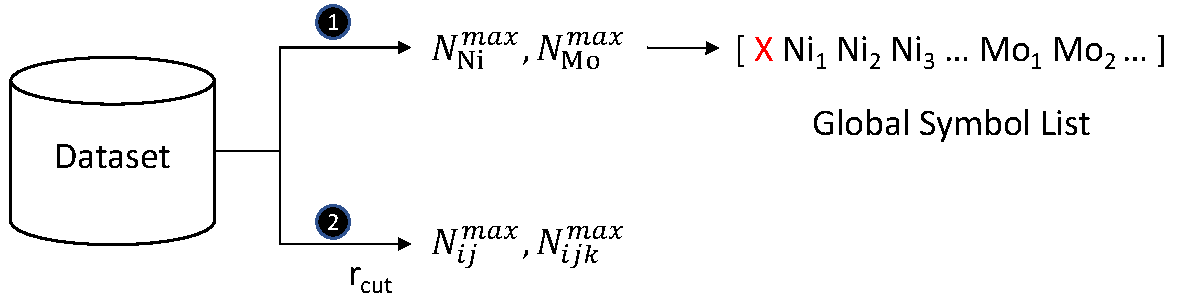
\includegraphics[scale=0.6]{figures/Fig2.pdf}
\caption{\label{fig:Fig2} The initialization step. 
\textbf{(1)} describes the detections of $N_{\mathrm{Ni}}^{\mathrm{max}}$, 
$N_{\mathrm{Ni}}^{\mathrm{max}}$ and the global symbol list (GSL). The red 'X' 
represents the inserted virtual atom.
\textbf{(2)} shows the detections of $\nijmax$ and $\nijkmax$ given $r_{cut}$.
}
\end{figure}

Fig \ref{fig:Fig2} shows the preparation stage of VAP. The cutoff radius 
$r_{cut}$ must be fixed. This stage has two major steps. The first step is to 
build the global symbol list (GSL), which acts as the universal reference 
system. A virtual atom is inserted at the very first position of GSL. 
To build GSL, all $\{\nelmax\}$ must be pre-determined where $\nelmax$ is the 
maximum appearances of element \textit{el} in any structure. $\nel$ represents 
the number of unique chemical elements in the dataset. Then, $\nvap$, the 
dimension of GSL, can be determined:
\begin{equation}
\label{eq:n_vap}
\nvap = 1 + \sum_{\mathrm{el}}{\nelmax}
\end{equation}
For the Ni-Mo dataset, $el \in [\mathrm{Ni}, \mathrm{Mo}]$ and 
$\nel = 2$. 
Table \ref{table:GSL} gives some examples of the GSL mapping. 'X' denotes the 
inserted virtual atom and Ni$_{108(54)}$ means the first 54 Ni atoms are mapped 
from the local stoichiometry. In the training phase, all $\nelmax$ are fixed.
In the prediction phase, $\nelmax$ shall be determined dynamically. One should 
note that the minimum value of $\nelmax$ should be 1 due to technical reason (so 
that the computation graph of TensorFlow can be properly executed). The codes to
get $\nelmax$ and GSL are given in Appendix(C). With GSL setup, atomic positions
and forces can be transformed as well. Appendix(D) gives the implementation of 
the virtual-atom mapping mechanism. 

% % % % % % % % % % % % % % % % % % % % % % % % % % % % % % % % % % % % % % % %
% 
% Table.1
%
% % % % % % % % % % % % % % % % % % % % % % % % % % % % % % % % % % % % % % % %
\begin{table}[h]
\centering
\begin{tabular}{lccccc}
\hline
 & Stoichiometry (Local) & $\nnimax$ & $\nmomax$ & $N^{\mathrm{vap}}$ 
 & Stoichiometry (GSL) \\
\hline
 & Ni$_{54}$ &  &  &  & XNi$_{108(54)}$Mo$_{176(0)}$ \\
Training & Ni$_{54}$Mo$_{12}$ & 108 & 176 & 285 
 & XNi$_{108(54)}$Mo$_{176(12)}$ \\
 & Mo$_{12}$ &  &  &  & XNi$_{108(0)}$Mo$_{176(12)}$ \\
\hline
 & Ni$_{54}$ & 54 & 1 & 56 & XNi$_{54(54)}$Mo$_{1(0)}$ \\
Prediction & Ni$_{54}$Mo$_{12}$ & 54 & 12 & 68 & XNi$_{54(54)}$Mo$_{12(12)}$ \\
 & Mo$_{12}$ & 1 & 12 & 14 & XNi$_{1(0)}$Mo$_{12(12)}$ \\
\hline
\end{tabular}
\caption{\label{table:GSL}
The mappings of local stoichiometries to their GSL forms, taking examples of the 
SNAP/Ni-Mo dataset.
}
\end{table}

Then we can determine another two key constants: $\nijmax$ and $\nijkmax$. 
Here $\nijmax$ represents the maximum number of atom-atom pairs in
arbitrary structure and the subscript 'ijk' denotes triples 
(or three-atoms) interactions. $\nijmax$ and $\nijkmax$ only depend on 
$r_{cut}$ and the associated codes are given in Appendix(B). 
Table \ref{table:nij_nijk_max} summarizes $\nijmax$ and $\nijkmax$ at different
$r_{cut}$ of the two demo datasets: QM7 and Ni-Mo (SNAP).

% % % % % % % % % % % % % % % % % % % % % % % % % % % % % % % % % % % % % % % %
% 
% Table.2
%
% % % % % % % % % % % % % % % % % % % % % % % % % % % % % % % % % % % % % % % %
\begin{table}[h]
\centering
\begin{tabular}{lccc}
\hline
 Dataset & $r_{cut}$(\AA) & $\nijmax$ & $\nijkmax$ \\
 QM7 & 6.5 & 506 & 5313 \\
\hline
 SNAP/Ni-Mo &  4.6 & 7200 & 176400 \\
 & 6.0 & 12384 & 526320 \\
 & 6.5 & 16284 & 965338 \\
\hline
\hline
\end{tabular}
\caption{\label{table:nij_nijk_max}
$\nijmax$ and $\nijkmax$ of SNAP/Ni-Mo and QM7 at different $r_{cut}$.
}
\end{table}

% % % % % % % % % % % % % % % % % % % % % % % % % % % % % % % % % % % % % % % %
% 
% Section 3.C
%
% % % % % % % % % % % % % % % % % % % % % % % % % % % % % % % % % % % % % % % %
\subsection{Interatomic distances}
\label{section:interatomic_distance}

% % % % % % % % % % % % % % % % % % % % % % % % % % % % % % % % % % % % % % % %
% 
% Fig.3
%
% % % % % % % % % % % % % % % % % % % % % % % % % % % % % % % % % % % % % % % %
\begin{figure}[h!]
\centering
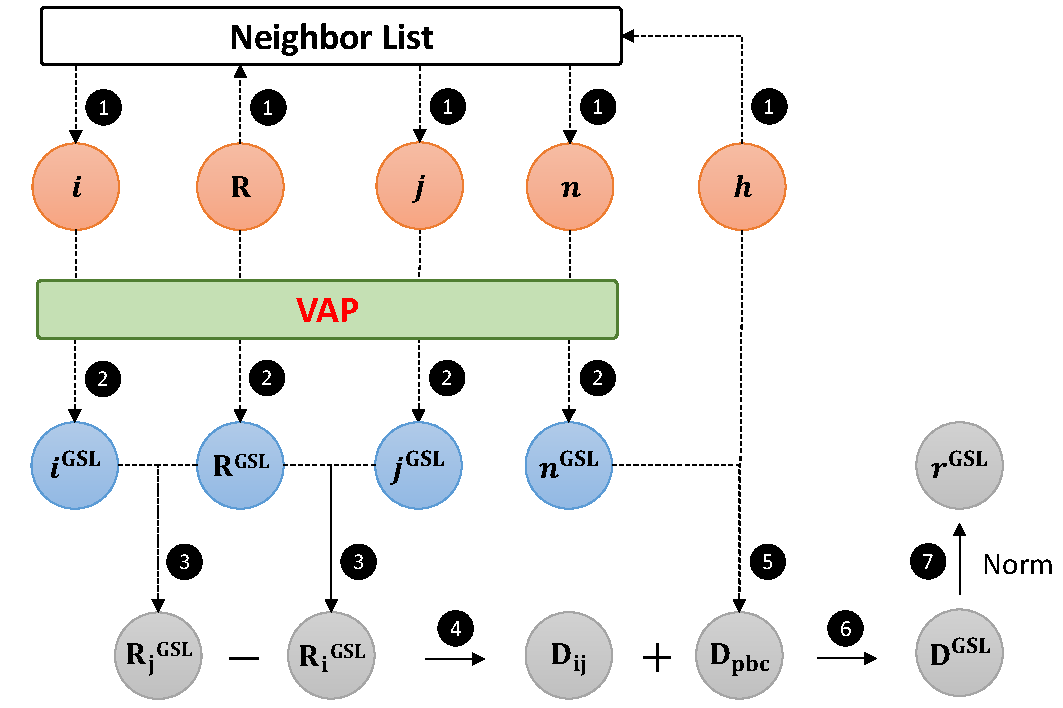
\includegraphics[scale=0.6]{figures/Fig3.pdf}
\caption{\label{fig:Fig3} The pseudo computation graph with execution orders for 
calculating interatomic distances $\mathbf{r}$ from atomic positions 
$\mathbf{R}$ and lattice tensor $\mathbf{h}$.
}
\end{figure}

Both the radial (Equation \ref{eq:g2}) and the angular (Equation \ref{eq:g4}) 
symmetry functions depends on interatomic distances only. In order to compute 
the descriptors, local atomic positions should be transformed to interatomic 
distances first. Fig \ref{fig:Fig3} demonstrates the pseudo graph of 
$\mathbf{R} \rightarrow \mathbf{r}^{\mathrm{GSL}}$ for radial symmetry function
descriptors: 

\begin{itemize}
    
    \item[1.] 
    Find all (i,j) neighbor pairs using the routine 
    \href{https://wiki.fysik.dtu.dk/ase/ase/neighborlist.html}
    {\textit{neighbor\_list}} implemented in ASE\cite{ase}. $\mathbf{R}$ 
    represents local atomic positions, $\mathbf{h}$ is the lattice tensor. 
    $\mathbf{i}$ and $\mathbf{j}$ are vectors of length $N_{\mathrm{ij}}$ and
    $\mathbf{n}$ is the $N_{\mathrm{ij}} \times 3$ periodic boundary shift 
    matrix. In the training phase $N_{\mathrm{ij}} \le \nijmax$; in the 
    prediction phase, $\nijmax$ is exactly equal to $N_{\mathrm{ij}}$.
    
    \item[2.] 
    Transform and expand local $\mathbf{R}$, $\mathbf{i}$, $\mathbf{j}$ and 
    $\mathbf{n}$ to their corresponding GSL arrays. These GSL arrays can be 
    cached for training. The transformations of $\mathbf{i}$, $\mathbf{j}$ and 
    $\mathbf{n}$ are straightforward: just appending $\nijmax - N_{ij}$ trailing 
    zeros. Fig \ref{fig:Fig3si} shows the mapping of 
    $\mathbf{R} \rightarrow \mathbf{R}^{\mathrm{GSL}}$ taking the example of 
    Ni$_3$Mo$_2$.

    \item[3.] 
    Broadcast $\mathbf{R}^{\mathrm{GSL}}$ to $\mathbf{R}_{i}^{\mathrm{GSL}}$ and
    $\mathbf{R}_{j}^{\mathrm{GSL}}$ with $\mathbf{i}^{\mathrm{GSL}}$ and 
    $\mathbf{j}^{\mathrm{GSL}}$ respectively.

    \item[4.]
    Compute the displacement vectors in the original cell:
    $\mathbf{D}_{ij} = \mathbf{j}^{\mathrm{GSL}} - \mathbf{i}^{\mathrm{GSL}}$
    
    \item[5.]
    Compute the periodic displacements:
    $\mathbf{D}_{pbc} = \mathbf{n}^{\mathrm{GSL}} \mathbf{h}$
    
    \item[6.]
    Compute the overall GSL displacements:
    $\mathbf{D}^{\mathrm{GSL}} = \mathbf{D}_{pbc} + \mathbf{D}_{ij}$
    
    \item[7.] 
    Compute the interatomic distances $\mathbf{r}^{\mathrm{GSL}}$ by calculating
    the 2-norm of each row of matrix $\mathbf{D}^{\mathrm{GSL}}$.

\end{itemize}

% % % % % % % % % % % % % % % % % % % % % % % % % % % % % % % % % % % % % % % %
% 
% Fig.3 (SI)
%
% % % % % % % % % % % % % % % % % % % % % % % % % % % % % % % % % % % % % % % %
\begin{figure}[h!]
\centering
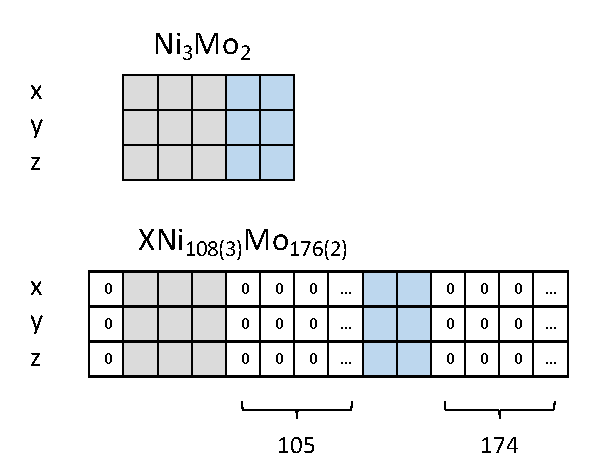
\includegraphics[scale=0.8]{figures/Fig3si.pdf}
\caption{\label{fig:Fig3si} The transformation of local $\mathbf{R}$ of 
Ni$_3$Mo$_2$ to $\mathbf{R}^{\mathrm{GSL}}$ of XNi$_{108(3)}$Mo$_{176(2)}$.
}
\end{figure}

Steps 1-2 are implemented in the function \textit{get\_g2\_map} in Appendix(E).
Steps 3-7 are implemented in the method \textit{get\_rij} of class 
\textit{SymmetryFunction} in Appendix(G). 

% % % % % % % % % % % % % % % % % % % % % % % % % % % % % % % % % % % % % % % %
% 
% Section 3.D
%
% % % % % % % % % % % % % % % % % % % % % % % % % % % % % % % % % % % % % % % %
\subsection{Radial descriptors}
\label{section:radial_descriptors}

Now we can start computing radial symmetry descriptors 
$\mathbf{G}^{(2)}$ from $\mathbf{r}^{\mathrm{GSL}}$. For simplicity, we will use 
the prediction phase to demonstrate this final section. 

Suppose we have $N_{\tau}$ different $(\eta, \omega)$ pairs for Equation 
\ref{eq:G2} and $(\eta, \omega)_{\tau} (0 \le \tau < N_{\tau})$ represents the 
$(\tau+1)$-th pair. In the prediction phase, $\mathbf{r}^{\mathrm{GSL}}$ should 
be a vector of length $\nijmax$ and the desired output $\mathbf{G}^{(2)}$ will 
be a matrix of shape $[\nvap, (\nel)^2 \cdot N_{\tau}]$, as shown in 
Fig \ref{fig:Fig5}\textbf{d}:
\begin{itemize}
    
    \item[1.] 
    The total number of rows is $\nvap$ (Equation \ref{eq:n_vap}) and each row
    represents the complete radial symmetry function descriptors of an atom. The 
    first row always corresponds to the inserted virtual atom.
    
    \item[2.]
    The total number of columns is $\nel \cdot \nel \cdot N_{\tau}$. Here 
    $\nel \cdot \nel$ indicates the number of element-element interaction types 
    and each interaction is described by $N_{\tau}$ feature values. For the 
    Ni-Mo dataset, there should be four unqiue interaction types: Ni-Ni, Ni-Mo, 
    Mo-Mo and Mo-Ni.

\end{itemize}

% % % % % % % % % % % % % % % % % % % % % % % % % % % % % % % % % % % % % % % %
% 
% Fig.4
%
% % % % % % % % % % % % % % % % % % % % % % % % % % % % % % % % % % % % % % % %
\begin{figure}[h!]
\centering
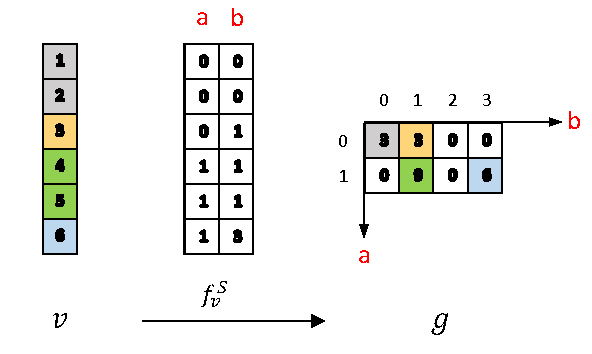
\includegraphics[scale=1.0]{figures/Fig4.pdf}
\caption{\label{fig:Fig4} The visualization of the mapping $f^S_{\nu}$.
In this example $S = [2,4]$ and $p$ can be any $(i,j)$ if 
$0 \le i < 2$ and $0 \le j < 4$.
}
\end{figure}

Assume $\nu$ is a vector of length $N_{\nu}$, we can define an integer matrix 
$f^{S}_{\nu}$ for mapping $\nu$ to a new array $g$ of shape $S$ satisfying the 
following conditions:
\begin{align}
\label{eq:scatter_nd}
% g(p) & = \sum_{\tau}^{}{\nu(\tau)}
g(p) & = \sum_{\tau=0}^{\tau < N_{\nu}}{c_\tau(p) \cdot \nu(\tau)} \\
c_{\tau}(p) & = \begin{cases}
    1 & {f^S}_{\nu}(\tau) = p \\
    0 & \mathrm{else}
\end{cases}
\end{align}
where $p$ is a coordinate vector. The matrix $f^{S}_{\nu}$ shall have $N_{\nu}$ 
rows and $N_S$ columns where $N_S$ represents the dimension of $g$. 
Fig \ref{fig:Fig4} visualizes this $f^S_{\nu}$ mapping scheme. This $f^S_{\nu}$
mapping plays a key role in transforming $\mathbf{r}^{\mathrm{GSL}}$ to 
$\mathbf{G}^{(2)}$.

% % % % % % % % % % % % % % % % % % % % % % % % % % % % % % % % % % % % % % % %
% 
% Fig.5
%
% % % % % % % % % % % % % % % % % % % % % % % % % % % % % % % % % % % % % % % %
\begin{figure}[h!]
\centering
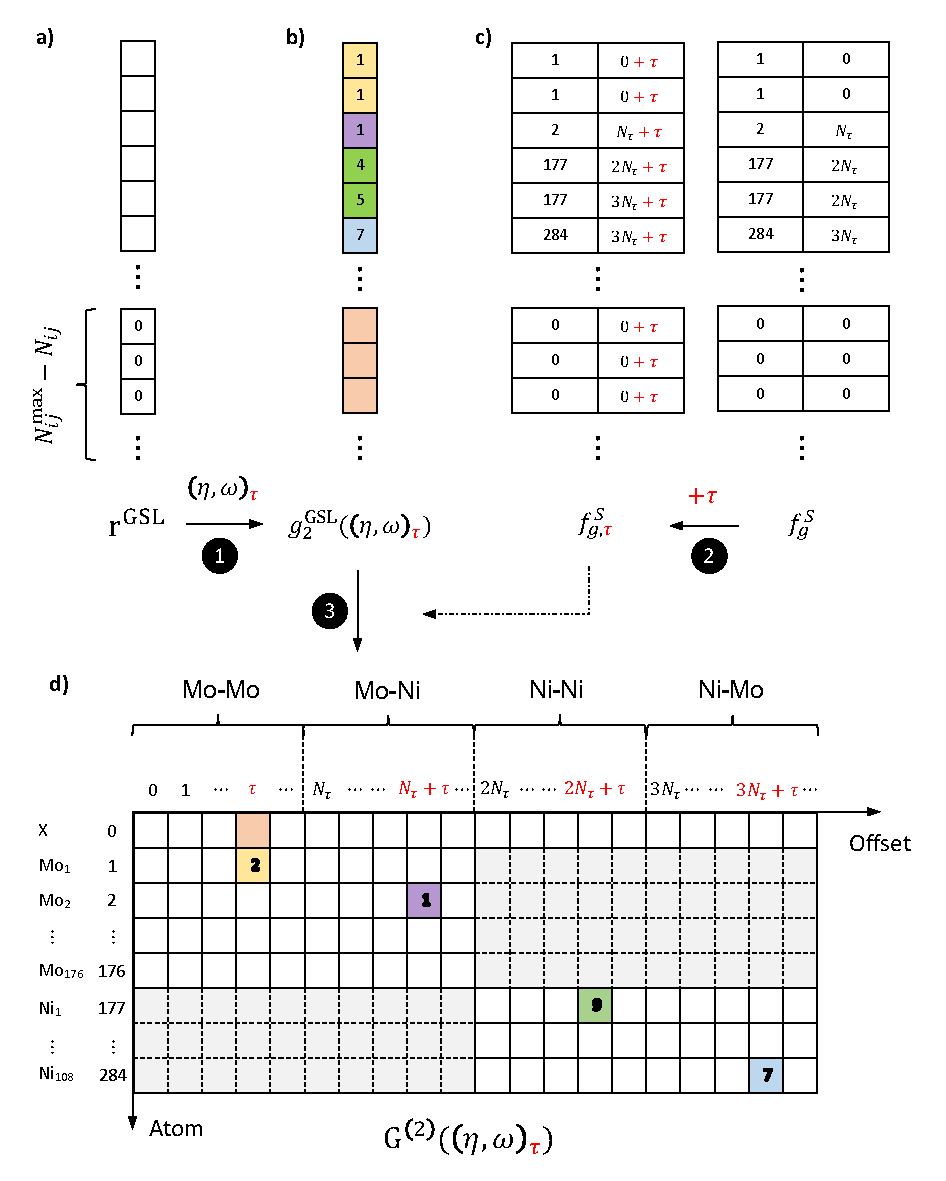
\includegraphics[scale=0.75]{figures/Fig5.pdf}
\caption{\label{fig:Fig5} The calculation of 
$\mathbf{G}^{(2)}((\eta, \omega)_{\tau})$ from $\mathbf{r}^{\mathrm{GSL}}$. 
}
\end{figure}

Fig \ref{fig:Fig5} 
demonstrates the calculation of $\mathbf{G}^{(2)}((\eta, \omega)_{\tau})$ from 
$\mathbf{r}^{\mathrm{GSL}}$. $\mathbf{G}^{(2)}((\eta, \omega)_{\tau})$ is the 
partial descriptors contributed by the $\tau$-th $(\eta, \omega)$ combination.
The overall $\mathbf{G}^{(2)}$ is just the sum of all partial contributions:
\begin{equation}
\mathbf{G}^{(2)} = \sum_{\tau=0}^{\tau < N_{\tau}}{
    \mathbf{G}^{(2)}((\eta, \omega)_{\tau})
}
\end{equation}
This calculation can be easily implemented with a \textit{For} loop. For each 
$\tau$, there will be three major steps:

\begin{itemize}
    
    \item[1.]
    The first step is applying Equation \ref{eq:g2} on 
    $\mathbf{r}^{\mathrm{GSL}}$ with the given $\tau$-th $(\eta, \omega)$ pair 
    to obtain $g^{\mathrm{GSL}}_{2}((\eta, \omega)_{\tau})$. 
    $g^{\mathrm{GSL}}_{2}((\eta, \omega)_{\tau})$ is a vector of length 
    $\nijmax$ and its last ($\nijmax - N_{ij}$) components are dummy values.
    
    \item[2.]
    The second step is generating the mapping $f_{g,\tau}^{S}$. In the Ni-Mo 
    case, $S=[285, 4N_{\tau}]$. $f_{g,\tau}^{S}$ is a matrix of shape 
    $[\nijmax, 2]$ and $f_{g,\tau}^{S}$ is constructed from the base mapping 
    array $f_{g}^{S}$ by adding $\tau$ to its second column. $f_{g}^{S}$ is also
    a $\nijmax \times 2$ matrix. $f_{g}^{S}$ stores fundamental properties of 
    $\mathbf{r}^{\mathrm{GSL}}$: the center atom (e.g. $\mathrm{Ni}_{1}$) and 
    type (e.g. Ni-Mo) of each atom-atom interaction:
    \begin{itemize}

        \item[a.] 
        Its first column is directly copied $i^{\mathrm{GSL}}$, representing the 
        GSL indices of the center atoms.
        
        \item[b.] 
        The values of its second column are multiples of $N_{\tau}$ indicating 
        the offsets, or horizontal positions in $\mathbf{G}^{(2)}$. These values 
        are obtained by multiplying $N_{\tau}$ with the type indices of 
        $\mathbf{r}^{\mathrm{GSL}}$. For example, the Ni-Mo dataset has two 
        unique elements: Ni, Mo. Hence, there will be four types of interactions:
        Mo-Mo (0), Mo-Ni (1), Ni-Ni (2) and Ni-Mo (3). Then for each value 
        (atom-atom interaction) of $\mathbf{r}^{\mathrm{GSL}}$, its type index 
        can be determined with $\mathbf{i}^{\mathrm{GSL}}$ and 
        $\mathbf{j}^{\mathrm{GSL}}$ based on the pre-built GSL.

    \end{itemize}
    
    \item[3.]
    Compute $\mathbf{G}^{(2)}((\eta, \omega)_{\tau})$ by applying 
    $f_{g,\tau}^{S}$ on $g^{\mathrm{GSL}}_{2}((\eta, \omega)_{\tau})$. The 
    padded zeros in $\mathbf{r}^{\mathrm{GSL}}$ are finally mapped to the 
    inserted virtual atom. Hence, the zero-padding of 
    $\mathbf{r}^{\mathrm{GSL}}$ can be easily separated and elinimated (just 
    remove the first row of $\mathbf{G}^{(2)}$). That's why TensorAlloy can use
    arbitrary number of structures without any stoichiometry restriction to do 
    batch training.

\end{itemize}

The mapping scheme $f_{\nu}^{S}$ can be directly achieved using routine 
\textit{tf.scatter\_nd} implemented by TensorFlow. The calculation of the base 
mapping array $f_{g}^{S}$ is implemented in Appendix(E). $f_{g}^{S}$ is also 
cacheable. The calculation of $\mathbf{G}^{(2)}((\eta, \omega)_{\tau})$ is 
implemented in method \textit{get\_g2\_op\_for\_tau} of class 
\textit{SymmetryFunction} in Appendix(G).

The workflow for the batch training phase is almost identical to the prediction 
phase described above. Meanwhile, there are some noticable diiferences:

\begin{itemize}
    
    \item[1.] 
    Most of the variables ($\mathbf{r}^{\mathrm{GSL}}$, 
    $\mathbf{i}^{\mathrm{GSL}}$, $\mathbf{R}^{\mathrm{GSL}}$, etc.) have one 
    more dimension. For example, $\mathbf{R}^{\mathrm{GSL}}$ should be an array
    of shape $[N_b, \nijmax, 3]$. Here $N_{b}$ represents the batch size.

    \item[2.]
    The atomic descriptors $\mathbf{G}^{(2)}$ becomes a 3D array of shape 
    $[N_b, \nvap, (\nel)^2 \cdot N_{\tau}]$.

    \item[3.] 
    The base mapping $f_{g}^{S}$ becomes a matrix of shape $[\nijmax, 3]$ in the 
    batch training phase. The newly inserted first column 
    \textemdash representing the batch indices \textemdash is 
    \textbf{not cacheable} because structures are selected randomly to form a 
    batch. Thus, the first column should be generated runtimely.

    \item[4.]
    In the training phase, $\nvap$ is a constant determined before training. In 
    the contrast, $\nvap$ should be a dynamic tensor 
    (or a \textit{tf.Placeholder} technically) in the prediction phase.
    Its value shall be runtimely determined according to the input structure. 

    \item[5.]
    In the training phase, the reference (or dft) atomic forces should be 
    transformed to GSL arrays before computing the loss contribution. The 
    NN-derived forces $\mathbf{F}^{\mathrm{NN}}$ are indeed GSL forces:
    \begin{equation}
        \mathbf{F}^{\mathrm{NN}} = 
        -\frac{\partial{E}}{\partial{\mathbf{R}^{\mathrm{GSL}}}}
    \end{equation}
    Hence, in the prediction phase, a reverse transformation should be applied 
    to obtain local \textbf{F}.

\end{itemize}

The training phase is implemented in \textit{BatchSymmetryFunction} which 
inherits most of methods from its parent class \textit{SymmetryFunction}. 
The dynamic batching scheme is implemented in method 
\textit{get\_v2g\_map\_batch\_indexing\_matrix}. The method 
\textit{get\_g\_shape} will return a fixed array instead. The function
\textit{map\_gsl\_array\_to\_local} of \textit{VirtualAtomMap} is used to do the 
reverse mapping.

% % % % % % % % % % % % % % % % % % % % % % % % % % % % % % % % % % % % % % % %
% 
% Section 3.E
%
% % % % % % % % % % % % % % % % % % % % % % % % % % % % % % % % % % % % % % % %
\subsection{Angular descriptors}

The same algorithm can be applied to compute angular symmetry function 
descriptors. The triple list shall be constructed from the neighbor list 
(Fig \ref{fig:Fig3}) and $\nijmax$ shall be replaced by $\nijkmax$. Typically
$\nijkmax \gg \nijmax$.

Appendix(F) demonstrates how to compute the base mapping array. The calculation 
of $\mathbf{G}^{(4)}(\beta, \gamma, \zeta)_{\tau}$ is implemented in method 
\textit{get\_g4\_op\_for\_tau} of class \textit{SymmetryFunction} 
in Appendix(G).

% % % % % % % % % % % % % % % % % % % % % % % % % % % % % % % % % % % % % % % %
% 
% Section 3.F
%
% % % % % % % % % % % % % % % % % % % % % % % % % % % % % % % % % % % % % % % %
\subsection{Min-max normalization}

Raw values of $\mathbf{G}^{(2)}$ and $\mathbf{G}^{(4)}$ may range from zero to 
several hundreds. So a min-max normalization routine is recommended. For each
column $\mathbf{G}(:, \tau)$ where $0 \le \tau < N_{\tau}$, we just normalize 
its values to range [0, 1]:
\begin{equation}
    \mathbf{G}(:, \tau) = \frac{
        \mathbf{G}(:, \tau) - \min(\mathbf{G}(:, \tau))}{
        \max(\mathbf{G}(:, \tau)) - \min(\mathbf{G}(:, \tau))}
\end{equation}
where $\min(\mathbf{G}(:, \tau))$ and $\max(\mathbf{G}(:, \tau))$ should be 
determined in the training phase and remain constant in the prediction phase. 

% % % % % % % % % % % % % % % % % % % % % % % % % % % % % % % % % % % % % % % %
% 
% Section 3.G
%
% % % % % % % % % % % % % % % % % % % % % % % % % % % % % % % % % % % % % % % %
\subsection{The residual model}

To fit the total energy, we slightly modified the total energy expression of 
Equation \ref{eq:general_e_total}:
\begin{align}
\label{eq:e_total_res}
E^{total} & = E^{residual} + E^{static} \nonumber \\
& = \sum_{\mathrm{el}}{\mathbf{NN}_{el}\left(\mathbf{G}_{\mathrm{el}}\right)}
+ \sum_{\mathrm{el}}{n_{el}E_{el}}
\end{align}
where $\{E_{el}\}$ is a set of \textit{trainable} scalar variables representing 
the \textit{static} energy of each type of element\cite{kCON}. The NN in 
Equation \ref{eq:e_total_res} just describes the atomistic interactions 
(the \textit{residual} energy). 
The introduction of $E^{static}$ can significantly limit value range of NN 
outputs, leading to faster convergence speed and higher training stability 
(Fig \ref{fig:benchmark_qm7}c). The initial $\{E_{el}\}$ are calculated by 
solving the linear system $Ax=b$ where $A$ is a $N_{data} \times \nel$ matrix 
and $b$ is a vector of length $N_{data}$. $N_{data}$ is the number of training 
examples. $A(i,j)$ is the number of $j$-th element in structure $i$ and $b(i)$ 
is the corresponding total energy.

In the training phase, the atomic descriptors array $\mathbf{G}^{(2)}$ is a 3D 
array because of the structure-based batching scheme. Thus, it's necessarily to 
use convolutional neural networks (CNNs) with 1x1 kernels\cite{kCON}. 
The traditional feed-forward neural networks with an additional 
atom-to-structure indexing\cite{Behler,ANI,TensorMol,DeePMD,BIMNN} are 
mathematically equivalent to CNNs with 1x1 kernels. However, using CNNs can make
the calculations of the \textit{automatically-differentiated per-structure} 
$\partial E/\partial \mathbf{R}$ and $\partial E/\partial \mathbf{h}$ much 
easier.

To train the model, we use the following root mean-squared error (RMSE) total 
loss function:
\begin{align}
\label{eq:loss}
\mathbf{Loss} & = \sqrt{\frac{1}{N_{b}}\sum_{i=1}^{N_{b}}{\left(
    E_{i} - E_{i}^{\mathrm{dft}}
\right)^2}} \nonumber \\
& + \chi_{\mathrm{f}}\sqrt{
    \frac{1}{3 N_{b} \nvap}\sum_{i}^{N_b}{\sum_{j}^{\nvap}{
        \sum_{\alpha}{
            \left(f_{ij\alpha} - f_{ij\alpha}^{\mathrm{dft}}\right)^2
        }
    }}
} \nonumber \\
& + \chi_{\mathrm{s}}\sqrt{\frac{1}{6N_b}\sum_{i}^{N_b}{
    \sum_{j}^{6}{
        \left(
            \epsilon^{\mathrm{voigt}}_{j} - \epsilon^{\mathrm{voigt,dft}}_{j}
        \right)^2
    }
}}
\end{align}
where $N_b$ is the mini-batch size and $\chi_{\mathrm{f}}$ and 
$\chi_{\mathrm{s}}$ are weights of force and virial losses. 
In most cases, we set $N_b$ to 50 or 100 and we
use the ADAM\cite{adam} optimizer with exponentially-decayed learning rate to 
minimize the loss function. The default activation function is softplus:
\begin{equation}
\sigma(x) = \log(1 + e^x)
\end{equation}
Softplus is a smooth approximation of the ReLU activation function.
The kernel weights of all NNs are initialized with the 
Xvaier method\cite{pmlr-v9-glorot10a} and kernel biases are initialized with 
zeros.

% % % % % % % % % % % % % % % % % % % % % % % % % % % % % % % % % % % % % % % %
% 
% Section 4. Results and Discussions
%
% % % % % % % % % % % % % % % % % % % % % % % % % % % % % % % % % % % % % % % %
\section{Results and Discussions}
\label{section:discussions}

In this section we demonstrate two experiments of TensorAlloy. All GPU benchmark
results are obtained on the same workstation with two Intel Xeon E5-2687v4 CPUs
(18 cores @ 2.3 GHz per CPU) and one NVIDIA GTX 1080Ti GPU.

% % % % % % % % % % % % % % % % % % % % % % % % % % % % % % % % % % % % % % % %
% 
% Section 4.A
%
% % % % % % % % % % % % % % % % % % % % % % % % % % % % % % % % % % % % % % % %
\subsection{QM7}

% % % % % % % % % % % % % % % % % % % % % % % % % % % % % % % % % % % % % % % %
% 
% Fig.6
%
% % % % % % % % % % % % % % % % % % % % % % % % % % % % % % % % % % % % % % % %
\begin{figure}[h!]
\centering
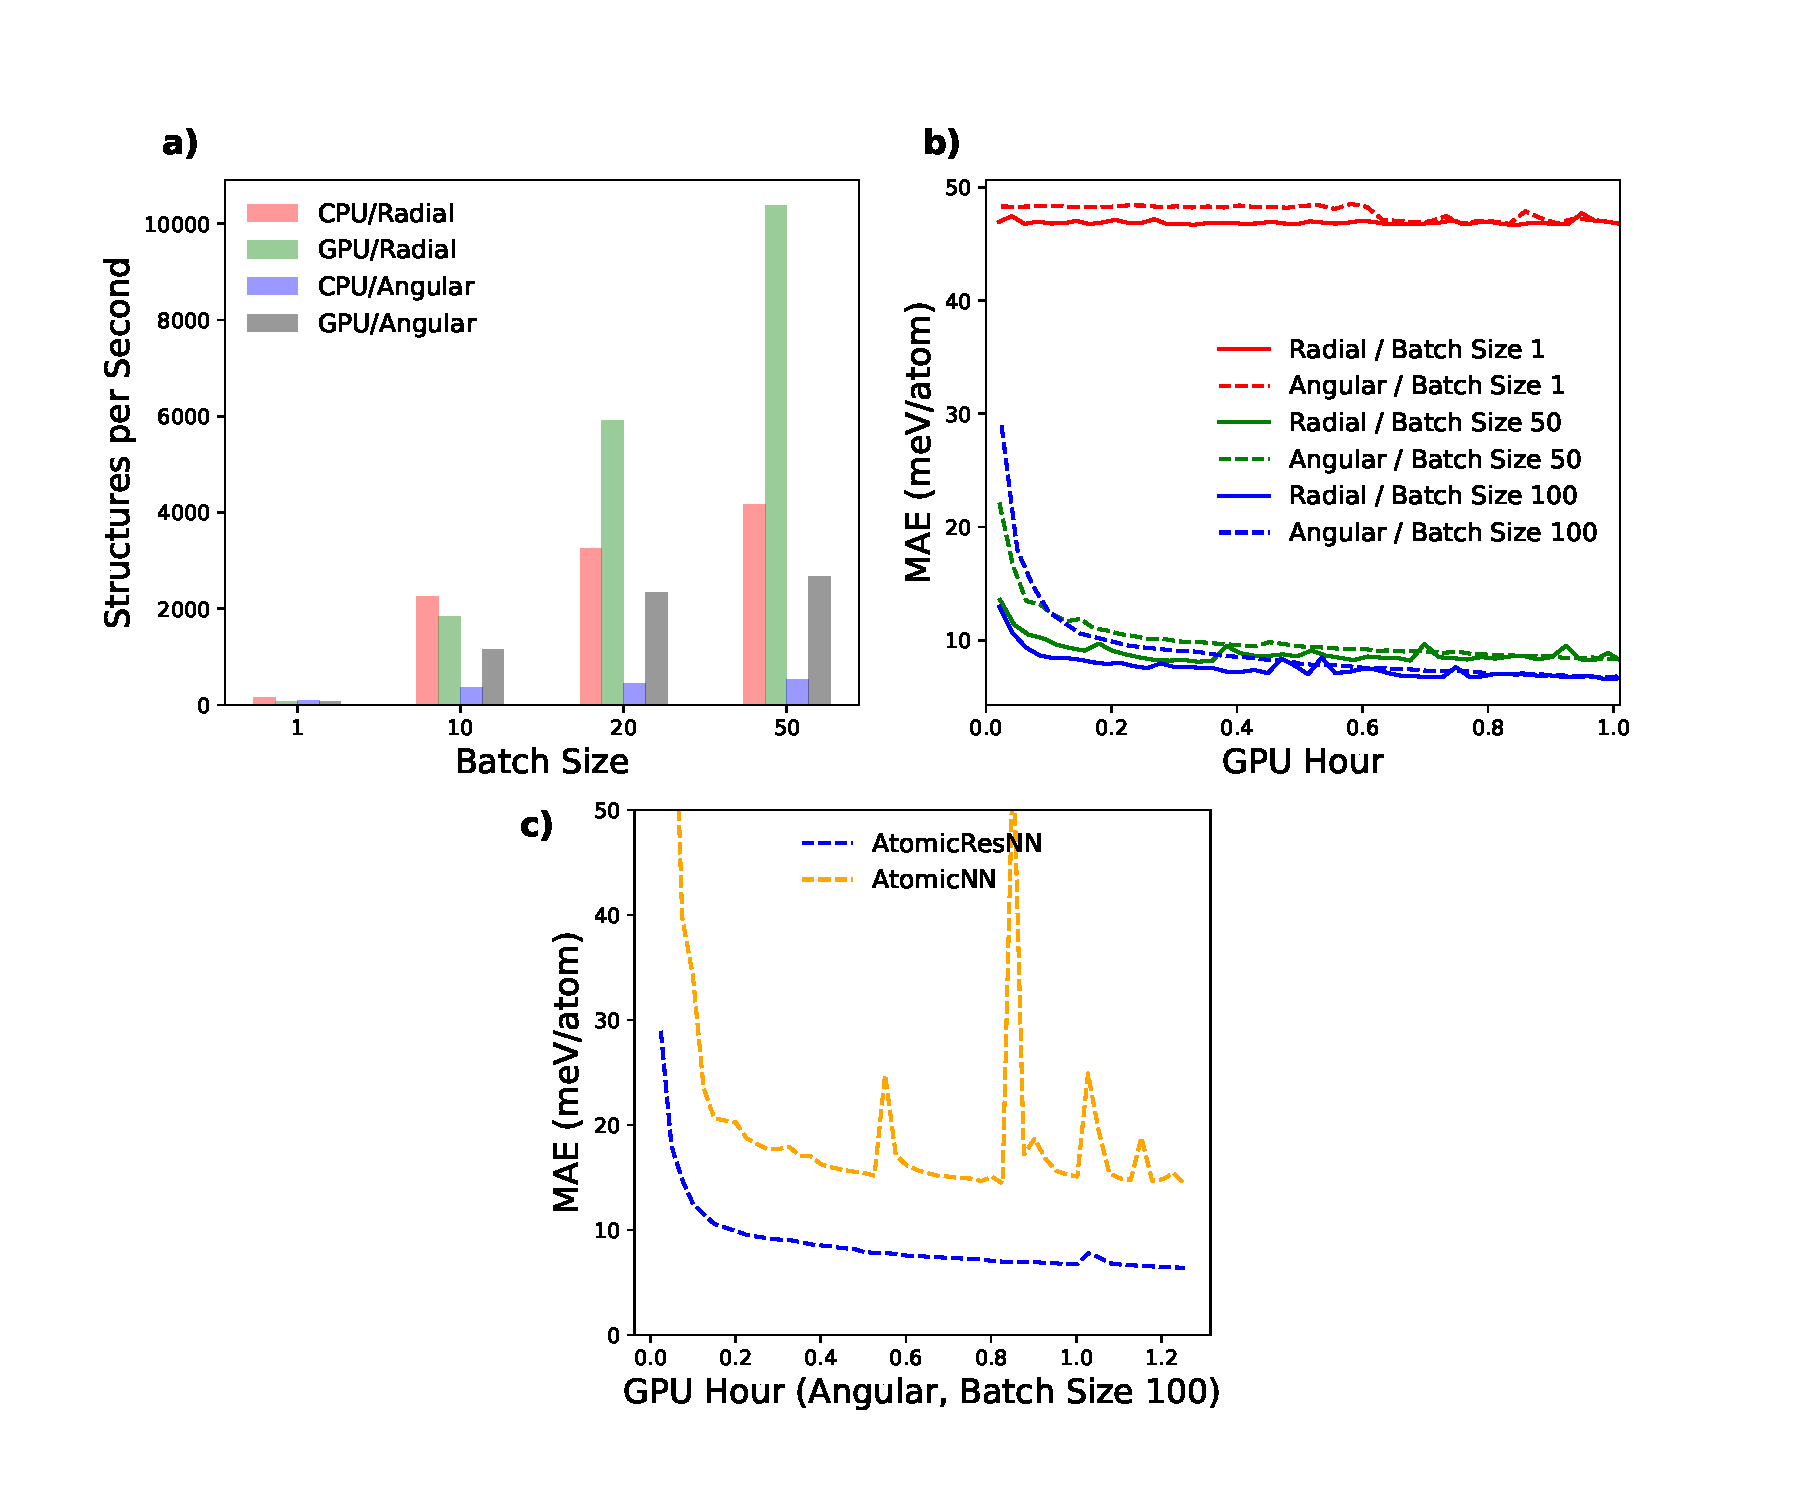
\includegraphics[scale=0.44]{figures/qm7_speed.pdf}
\caption{\label{fig:benchmark_qm7} 
\textbf{a)} The curves of training speed (structures per second) vs batch sizes. 
\textbf{b)} The curves of test MAE (meV/atom) vs training time (GPU hour) using 
different settings.
\textbf{c)} The curves of test MAE (meV/atom) vs NN models. 
}
\end{figure}

QM7\cite{QM7_1,QM7_2} is a publicly available benchmark dataset calculated at 
the DFT level. The QM7 dataset contains 7165 stable organic molecules 
(C, H, N, O, S) with 176 unique stoichiometries. The total energies range from 
-95 eV to -17 eV and the structure sizes range from 5 to 23. 1000 structures 
were randomly selected as test set before training.

Figure \ref{fig:benchmark_qm7} demonstrates the performances of 
TensorAlloy on QM7 dataset. In this figure, 'Radial' means only radial 
symmetry functions (Equation \ref{eq:G2}) are used and 'Angular' indicates both 
radial and angular symmetry functions are used. The cutoff radius is 6.5 \AA.
The corresponding $\nijmax$ and $\nijkmax$ are 506 and 5313, respectively.
Values of $\eta$ for radial symmetry functions are 0.1, 0.5, 1, 2, 4, 8, 12, 16, 
20, 40 and $\beta$ (0.1, 0.5), $\gamma$ (1, -1) and $\zeta$ (1, 4) are used for
angular functions. $\omega$ is fixed to 0. The initial learning rate is 0.01. 
Learning rate decay is disabled for the following tests. Min-max normalization
is enabled. Each atomistic neural network has two hidden layers with 64 and 32 
neurons. The force and stress losses of Equation \ref{eq:loss} are disabled for 
this experiment.

Figure \ref{fig:benchmark_qm7}a compares the training speed (number of processed 
structures per second) with different batch sizes (number of structures per 
step). It shows that CPU perfers fewer descriptors (radial only) and smallber 
batch size while GPU is suitable for larger batch size and more complicated 
descriptors (radial + angular). 
Figure \ref{fig:benchmark_qm7}b shows the curves of mean absolute errors 
(MAEs, meV/atom) on the test set. This figure clearly illustrate another benefit 
of using larger batch size: the trainings can be much faster. For the best case 
(batch size 100, angular symmetry functions included), the test MAE will reach 6 
meV/atom (1.8 kcal/mol per structure) in just one GPU hour on our workstation.

Figure \ref{fig:benchmark_qm7}c compares out residual model (Equation 
\ref{eq:e_total_res}) with traditional ANN model (Equation 
\ref{eq:general_e_total}). The proposed residual model has a much faster 
convergence rate and better stability. One exaplanation is that the 
\textit{static} part acts as a normalization function. By introducing the 
\textit{static} term, the output values of ANNs are much closer to the ideal 
output range (-1, 1) of neural networks.

% % % % % % % % % % % % % % % % % % % % % % % % % % % % % % % % % % % % % % % %
% 
% Section 4.B
%
% % % % % % % % % % % % % % % % % % % % % % % % % % % % % % % % % % % % % % % %
\subsection{Ni-Mo}

SNAP/Ni-Mo\cite{SNAP_Mo_2017, SNAP_2018} is a publicly available dataset built 
by Shyue Ping Ong and co-workers. This dataset has 3971 Ni-Mo solids, including 
461 pure Ni structures and 284 pure Mo structures. All DFT calculations were 
done by VASP\cite{VASP} using the PBE\cite{PBE} functional within the projector 
angumented-wave (PAW)\cite{PAW} approach.

In this experiment, we trained three different models:
\begin{enumerate}
    
    \item \textbf{NN}(Ni): this model uses 400 Ni structures for training and 61 
    for evaluation. The loss function only includes energy and force 
    contributions.
    
    \item \textbf{NN}(Mo): this model uses 250 Mo structures for training and 34 
    for evaluation. The loss function includes all three (energy, force, stress) 
    types of contributions. 
    
    \item \textbf{NN}(Mo-Ni): this model uses 3673 structures for training and 
    300 for evaluation. The loss function includes all three types of 
    contributions.

\end{enumerate}

The cutoff radius is set to 6.5 \AA. Only radial symmetry 
functions are used to compute atomic descriptors. The selected $\eta$ are 
0.1, 0.5, 1, 2, 4, 8, 12, 16, 20, 40 and $\omega$ are 0.0, 3.0. The hidden layer
sizes are 128, 64, 32. The activation function is softplus.
The learning rate starts from 0.01 and it will decay exponentially with rate 
0.95 for every 3000 steps.

% % % % % % % % % % % % % % % % % % % % % % % % % % % % % % % % % % % % % % % %
% 
% Table. 3
%
% % % % % % % % % % % % % % % % % % % % % % % % % % % % % % % % % % % % % % % %
\begin{table}[h]
\centering
\begin{tabular}{cccc}
\hline
\multicolumn{4}{c}{Binary Mo-Ni model} \\
\hline
Subset & Energy (meV/atom) & Force (eV/\AA) & Stress (GPa) \\
\hline
Mo & 16.5 (16.2) & 0.28 (0.29) & 0.75 \\
Ni & 4.5 (7.9)   & 0.07 (0.11) & 0.83 \\
Ni$_4$Mo & 4.1 (4.0) & 0.09 (0.14) & 0.98 \\ 
Ni$_3$Mo & 4.5 (5.2) & 0.11 (0.16) & 1.19 \\
Ni$_{\mathrm{Mo}}$ & 12.9 (22.7) & 0.09 (0.13)& 0.34 \\
Mo$_{\mathrm{Ni}}$ & 12.9 (33.9) & 0.12 (0.55)& 0.45 \\
Overall & 10.8 (22.5)& 0.11 (0.23) & 0.59 \\
\hline
\end{tabular}
\caption{\label{table:MAE}
Comparion of the MAEs in predicted energies (mev/atom), forces (eV/\AA) and 
stress (GPa) relative to DFT of each subset for the binary Mo-Ni model and the
corresponding SNAP benchmarks (bracket)}
\end{table}

\begin{table}[h]
\centering
\begin{tabular}{ccc|cc|c}
\hline
  & \multicolumn{2}{c|}{Energy (meV/atom)} & \multicolumn{2}{c|}{Force (eV/\AA)}
  & Stress (GPa) \\
\hline
Elementary Model & Mo         & Ni        & Mo            & Ni   & Mo          \\
\hline
Mo               & 4.5 (13.2) &           & 0.19 (0.25)   &      & 0.28 (0.87) \\
Ni               &            & 1.3 (1.2) & & 0.04 (0.05) & 2.05               \\
\hline
\end{tabular}
\caption{\label{table:MAE1}
Comparion of the MAEs in predicted energies (mev/atom), forces (eV/\AA) and 
stress (GPa) relative to DFT for the two elementary models (Ni, Mo) and their
corresponding SNAP benchmarks (bracket)}
\end{table}

Table \ref{table:MAE} and \ref{table:MAE1} summarizes the energy, force and 
stress prediction performances of our trained models compared with their 
corresponding SNAP benchmarks. 
The original SNAP formalism contains both radial and angular 
interactions. However, in most cases, the radial-only TensorAlloy-trained 
models can significantly outperform corresponding SNAP models. We can also 
notice that including virial stress in the total loss function can significantly
reduce the stress prediction error. The virial stress 
(Equation \ref{eq:stress}) consists of two parts: the net force contribution 
$-F^TR$ and the partial force contribution 
$\left(\partial E / \partial \mathbf{h}\right)^T\mathbf{h}$. The atomic forces 
used by the total loss equation \ref{eq:loss} are net forces only but virial 
stress only depends on the partial forces (the force between two atoms). 
Compared with the binary \textbf{NN}(Mo-Ni) model, the elementary 
\textbf{NN}(Ni) model has lower net force error (0.04 eV/\AA vs 0.07 eV\AA). 
However, the elementary model trained with energy and forces only has much 
larger stress MAE (2.05 GPa vs 0.83 GPa). These results clearly suggest that 
including virial stress in the total loss function is necessary for obtaining 
better virial stress accuracy.

% % % % % % % % % % % % % % % % % % % % % % % % % % % % % % % % % % % % % % % %
% 
% Fig.7
%
% % % % % % % % % % % % % % % % % % % % % % % % % % % % % % % % % % % % % % % %
\begin{figure}[h!]
    \centering
    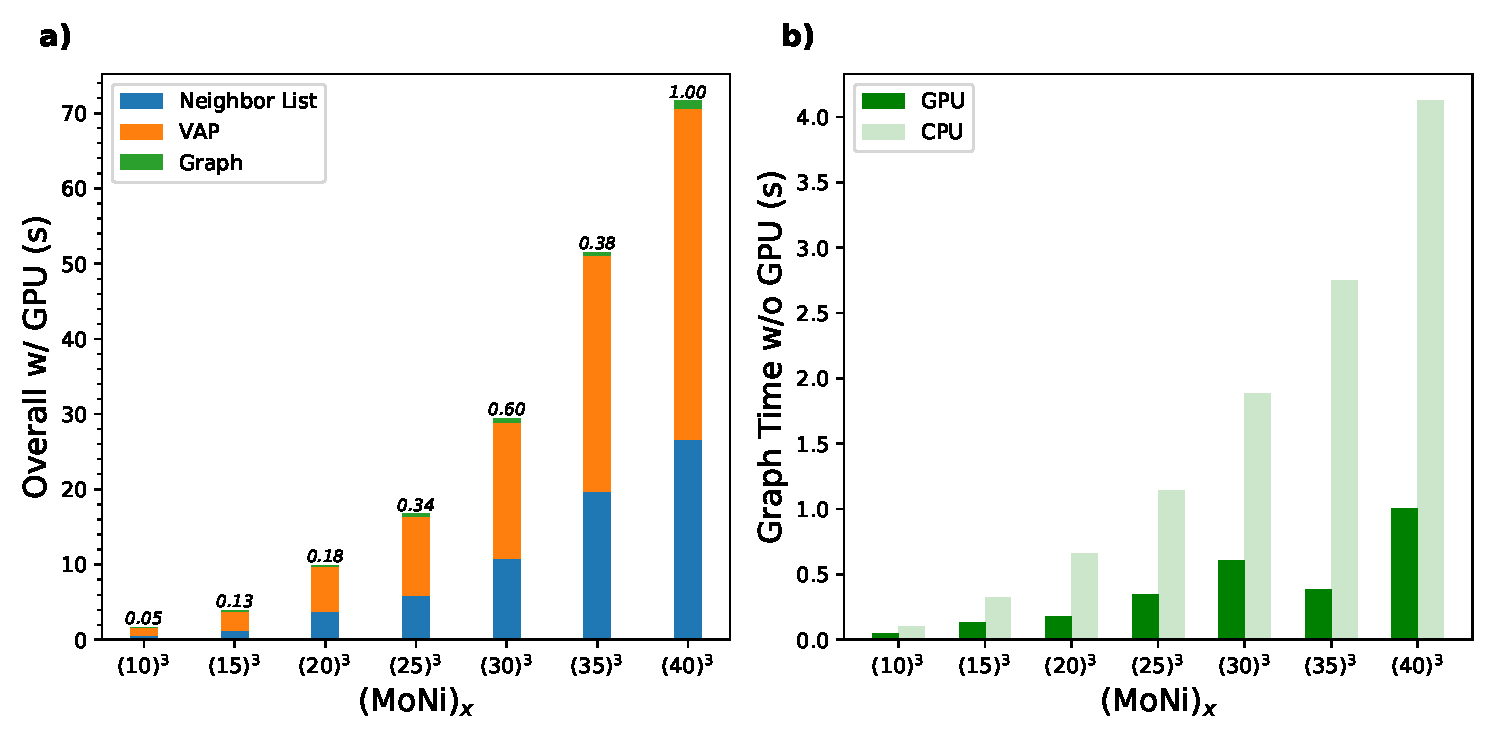
\includegraphics[scale=0.5]{figures/Prediction-speed.pdf}
\caption{\label{fig:prediction_speed} Benchmarks of the \textbf{NN}(Mo-Ni) model 
in the prediction phase. The test structures are (MoNi)$_{x}$ where 
$x$ = $10^3, 15^3, 20^3, 25^3, 30^3, 35^3, 40^3$. The left figure \textbf{a)} 
demonstrates the overall time and the right figure \textbf{b)} compares the 
'Graph' time with/out GPU. Blue bars indicate the elapsed time (in seconds) for 
finding neighbors, orange bars denote the time for initializing VAP-GSL arrays 
and green bars and the numbers above represents the graph execution time (used 
for obtaining energy, forces and stress).
}
\end{figure}

The speed of the prediction phase is also a crucial metric for measuring 
interaction potentials. Fig \ref{fig:prediction_speed} summarizes the time 
distribution of the \textbf{NN}(Ni-Mo) model in the prediction phase on the GPU 
workstation. 
Here 'prediction' is defined as calculating energy, forces and stress tensor of 
an arbitrary \textit{ase.Atoms} object. In these tests, the primitive structure
$\mathrm{MoNi}$ is obtained by replacing one of the two bcc Mo atoms with a Ni 
atom. The test subjects $(\mathrm{MoNi}))_{x}$ are just supercells of the base 
structure. We choose $x \in [10^3, 15^3, 20^3, 25^3, 30^3, 35^3, 40^3]$ as
a typical molecular dynamics simulation for studying alloy properties needs at 
least thousands of atoms. The elaspsed time is splitted to three parts: 
'Neighbor' (blue) indicates the execution time of the \textit{neighbor\_list} 
routine of ASE for finding local neighbors (\textbf{(1)} of Fig \ref{fig:Fig3}),
'VAP' (orange) denotes the time to construct VAP-GSL arrays 
(\textbf{(2)} of Fig \ref{fig:Fig3}) and 'Graph' (green bars and the numbers 
above) represents the time of getting energy, forces and stress tensor by 
executing the computation graph. The smallest subject (2000 atoms) needs 1.6 
seconds and the largest system (128000 atoms) requires ~71.6 seconds on the 
workstation. Most of the time are spent on the Python-based single-thread 
'Neighbor' and 'VAP' routines \textemdash which may be greatly optimized by 
utilizing efficient C/C++/Fortran codes (e.g. Lammps). For the 'Graph' part, the 
execution time can be as small as 1 second (with GPU) or 4 seconds (without GPU) 
for the 128000-atoms structure. According to these tests, it's fairly practical 
to use TensorAlloy-trained symmetry function interaction potential on studying 
large alloy systems.

% % % % % % % % % % % % % % % % % % % % % % % % % % % % % % % % % % % % % % % %
% 
% Fig.8
%
% % % % % % % % % % % % % % % % % % % % % % % % % % % % % % % % % % % % % % % %
\begin{figure}[h!]
    \centering
    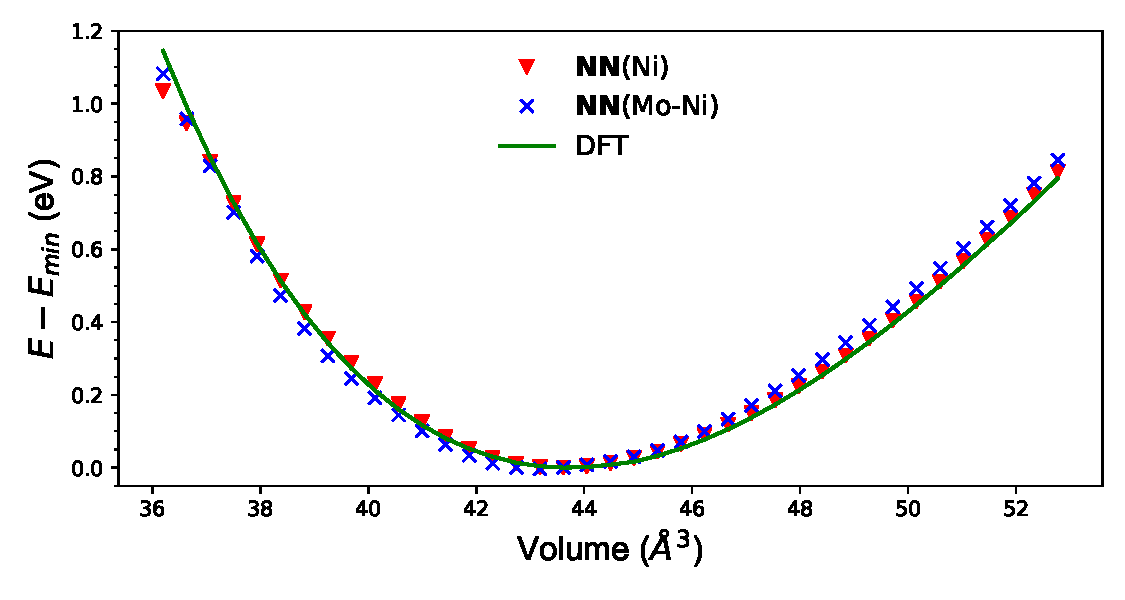
\includegraphics[scale=0.65]{figures/Ni_EoS.pdf}
\caption{\label{fig:energy_volume_Ni} The energy vs volume curves of fcc Ni for
the DFT, Ni and Ni-Mo models.}
\end{figure}

To further validate our models, we also calculate the energy-volume curves of a 
conventional fcc Ni cell using \textbf{NN}(Ni) and \textbf{NN}(Mo-Ni) models. 
The results are plotted in Fig \ref{fig:energy_volume_Ni}. Both curves overlap 
the DFT curve very well in the range of -17\% to 21\% from the equilibrium 
volume. The surface energy tests, as shown in Fig \ref{fig:surface_energy_Ni}, 
also proves the accuracy of TensorAlloy-optimized models. 
PyMatGen\cite{pymatgen,pymatgen-1} is used to generate these surface slabs.

% % % % % % % % % % % % % % % % % % % % % % % % % % % % % % % % % % % % % % % %
% 
% Fig.9
%
% % % % % % % % % % % % % % % % % % % % % % % % % % % % % % % % % % % % % % % %
\begin{figure}[h!]
    \centering
    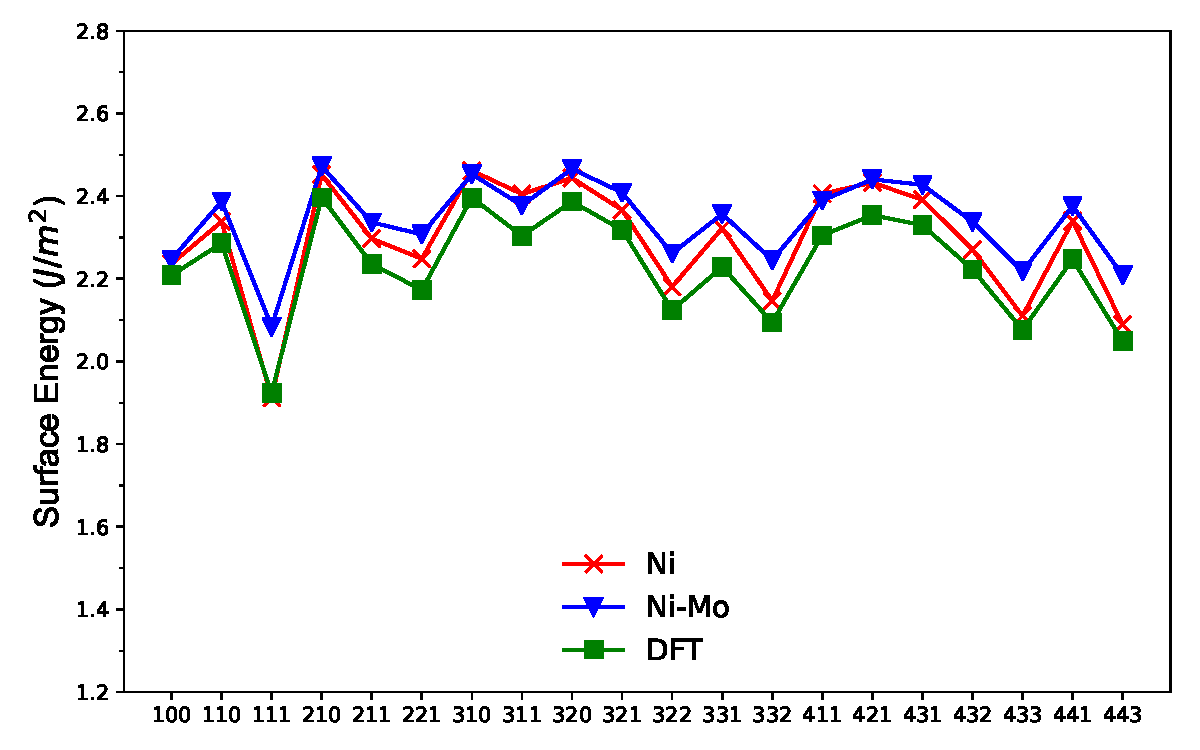
\includegraphics[scale=0.65]{figures/Ni_surface_energy.pdf}
\caption{\label{fig:surface_energy_Ni} Surface formation energies ($J/m^2$) of 
different Ni surfaces calculated by DFT, Ni and Ni-Mo models}
\end{figure}

% % % % % % % % % % % % % % % % % % % % % % % % % % % % % % % % % % % % % % % %
% 
% Section 5. Conclusions
%
% % % % % % % % % % % % % % % % % % % % % % % % % % % % % % % % % % % % % % % %
\section{Conclusions}
\label{section:conclusions}

In this work, we introduced our virtual atom approach and a smart way of 
constructing symmetry function based atomistic neural networks. 
With the virtual atom approach, the calculations of the symmetry function 
descriptors can be implemented within TensorFlow. Thus, we can now build direct 
computation graph from atomic positions to total energy, making the technical 
barrier of calculating NN-derived atomic forces and virial stress neglectable.
This new algorithm is implemented in our Python program, TensorAlloy.

% % % % % % % % % % % % % % % % % % % % % % % % % % % % % % % % % % % % % % % %
% 
% Acknowledgments
%
% % % % % % % % % % % % % % % % % % % % % % % % % % % % % % % % % % % % % % % %
\section*{Acknowledgments}

This work was supported by the National Key Research and Development Program of 
China under Grant No. 2016YFB0201204, the Science Challenge Project under Grant 
No. TZ2018002 and the National Natural Science Foundation of China under Grant 
No. U1630250.

% % % % % % % % % % % % % % % % % % % % % % % % % % % % % % % % % % % % % % % %
% 
% References
%
% % % % % % % % % % % % % % % % % % % % % % % % % % % % % % % % % % % % % % % %

\bibliographystyle{elsarticle-num}
\bibliography{manuscript.bib}

% % % % % % % % % % % % % % % % % % % % % % % % % % % % % % % % % % % % % % % %
% 
% Appendix
%
% % % % % % % % % % % % % % % % % % % % % % % % % % % % % % % % % % % % % % % %
\section*{Appendix}
\label{section:appendix}

% % % % % % % % % % % % % % % % % % % % % % % % % % % % % % % % % % % % % % % %
% 
% Section Appendix. A
%
% % % % % % % % % % % % % % % % % % % % % % % % % % % % % % % % % % % % % % % %
\subsection{Derivation and implementation of the virial stress equation}

According to Equation \ref{eq:lattice} and Equation \ref{eq:ij_shift}, Equation 
\ref{eq:rijn} can be expanded:
\begin{align}
\rijn = & \Vert \mathbf{r}_i^{(0)} - \mathbf{r}_j^{(0)} + 
           \mathbf{n}^T \mathbf{h} \Vert \nonumber \\
      = & \left[
                 \left(r_{j,x}^{(0)} - r_{i,x}^{(0)} + 
                       \sum_{\alpha}{n_{\alpha}h_{\alpha x}} \right)^2 +
                 \left(r_{j,y}^{(0)} - r_{i,y}^{(0)} + 
                       \sum_{\alpha}{n_{\alpha}h_{\alpha y}} \right)^2 + \right.
        \nonumber \\
        & \left. \left(r_{j,z}^{(0)} - r_{i,z}^{(0)} + 
                       \sum_{\alpha}{n_{\alpha}h_{\alpha z}} \right)^2 
          \right]^{\frac{1}{2}}
\end{align}
where $\alpha=x,y,z$. Thus, we can calculate the derivation of $\rijn$ with 
respect to $h_{\alpha\beta}$:
\begin{gather}
\frac{\partial \rijn}{\partial h_{\alpha\beta}} = 
    \frac{1}{\rijn} \cdot \Delta_{ij\mathbf{n}\beta} \cdot n_{\alpha} \\
\Delta_{ij\mathbf{n}\beta} = r_{j,\beta}^{(0)} - r_{i,\beta}^{(0)} + 
    \sum_{\alpha}{n_{\alpha}h_{\alpha \beta}}
\end{gather}

\newcommand{\hab}{h_{\alpha\beta}}
\newcommand{\hga}{h_{\gamma\alpha}}
\newcommand{\hgb}{h_{\gamma\beta}}

Then we can derive $\partial E^{total} / \partial \hab$:
\begin{align}
\label{eq:dEdhab}
\frac{\partial E^{total}}{\partial \hab} = \sum_{i}^{N}{\sum_{l}^{N_G}}{
    \frac{\partial \mathbf{NN}_{el}(\mathbf{G}_i)}{\partial G_{il}}
    \cdot
    \frac{\partial G_{il}}{\partial \hab}
}
\end{align}
If $G_{il}$ is a radial symmetry function:
\begin{align}
\frac{\partial G_{il}^{(2)}}{\partial \hab} 
& = \sum_{j \neq i}{\sum_{\mathbf{n}}}{
    \frac{\partial g_2}{\partial \rijn} 
    \cdot 
    \frac{1}{\rijn} \cdot \Delta_{ij\mathbf{n}\beta} \cdot n_{\alpha}
} \\
\label{eq:stress_g2_right}
\frac{\partial G_{il}^{(2)}}{\partial \hga} \cdot \hgb & = 
\sum_{j \neq i}{\sum_{\mathbf{n}}}{
    \frac{\partial g_2}{\partial \rijn} 
    \cdot 
    \frac{\Delta_{ij\mathbf{n}\alpha}}{\rijn} \cdot n_{\gamma}
} \cdot \hgb
\end{align}
If $G_{il}$ is an angular symmetry function:
\begin{align}
\frac{\partial G_{il}^{(4)}}{\partial \hab} & =
    \sum_{j, k \neq j, k \neq i}{
        \sum_{\mathbf{n_1}}}{\sum_{\mathbf{n_2}}{\sum_{\mathbf{n_3}}{
    \left(
        \frac{\partial g_4}{\partial \rijna}\cdot\frac{\partial \rijna}{\hab} +
        \frac{\partial g_4}{\partial \rikna}\cdot\frac{\partial \rikna}{\hab} +
        \frac{\partial g_4}{\partial \rjkna}\cdot\frac{\partial \rjkna}{\hab}
    \right)
}}} \nonumber \\
& =  \sum_{j, k \neq j, k \neq i}{
        \sum_{\mathbf{n_1}}}{\sum_{\mathbf{n_2}}{\sum_{\mathbf{n_3}}{
    \frac{\partial g_4}{\partial \rijna} \cdot 
    \frac{\Delta_{ij\mathbf{n_1}\beta}}{\rijna} \cdot n_{1,\alpha}
}}} \nonumber \\
& + \sum_{j, k \neq j, k \neq i}{
    \sum_{\mathbf{n_1}}}{\sum_{\mathbf{n_2}}{\sum_{\mathbf{n_3}}{
\frac{\partial g_4}{\partial \rikna} \cdot 
\frac{\Delta_{ik\mathbf{n_2}\beta}}{\rikna} \cdot n_{2,\alpha}
}}} \nonumber \\
& + \sum_{j, k \neq j, k \neq i}{
    \sum_{\mathbf{n_1}}}{\sum_{\mathbf{n_2}}{\sum_{\mathbf{n_3}}{
\frac{\partial g_4}{\partial \rjkna} \cdot 
\frac{\Delta_{jk\mathbf{n_2}\beta}}{\rjkna} \cdot n_{3,\alpha}
}}} \\
\label{eq:stress_g4_right}
\frac{\partial G_{il}^{(4)}}{\partial \hga} \cdot \hgb & = 
\sum_{j, k \neq j, k \neq i}{
    \sum_{\mathbf{n_1}}}{\sum_{\mathbf{n_2}}{\sum_{\mathbf{n_3}}{
\frac{\partial g_4}{\partial \rijna} \cdot 
\frac{\Delta_{ij\mathbf{n_1}\alpha}}{\rijna} \cdot n_{1,\gamma} \cdot \hgb
}}} \nonumber \\
& + \sum_{j, k \neq j, k \neq i}{
    \sum_{\mathbf{n_1}}}{\sum_{\mathbf{n_2}}{\sum_{\mathbf{n_3}}{
\frac{\partial g_4}{\partial \rikna} \cdot 
\frac{\Delta_{ik\mathbf{n_1}\alpha}}{\rikna} \cdot n_{2,\gamma} \cdot \hgb
}}} \nonumber \\
& + \sum_{j, k \neq j, k \neq i}{
    \sum_{\mathbf{n_1}}}{\sum_{\mathbf{n_2}}{\sum_{\mathbf{n_3}}{
\frac{\partial g_4}{\partial \rjkna} \cdot 
\frac{\Delta_{jk\mathbf{n_1}\alpha}}{\rjkna} \cdot n_{3,\gamma} \cdot \hgb
}}}
\end{align}
Combining with Equation \ref{eq:dEdhab}, \ref{eq:stress_g2_right} and 
\ref{eq:stress_g4_right}, we can now start deriving the right part of Equation 
\ref{eq:stress}. To simplify the derivation, we just assume $G_{il}$ represents
a radial function:
\newcommand{\dE}{\partial{E^{total}}}
\begin{align}
\label{eq:dEdhTh_g2_expanded}
\left(
    \left(\frac{\partial E^{total}}{\partial \mathbf{h}}\right)^T \mathbf{h}
\right)_{\alpha\beta} & = 
\sum_{\gamma}{\frac{\dE}{\partial \hga} \hgb} \nonumber \\
& = \sum_{\gamma}{\sum_{i}^{N}{\sum_{l}^{N_G}}{
    \frac{\partial \mathbf{NN}_{el}(\mathbf{G}_i)}{\partial G_{il}}
    \cdot
    \sum_{j \neq i}{\sum_{\mathbf{n}}}{
    \frac{\partial g_2}{\partial \rijn} 
    \cdot 
    \frac{\Delta_{ij\mathbf{n}\alpha}}{\rijn} \cdot n_{\gamma}} \hgb
}} \nonumber \\
& = \sum_{i}^{N}{\sum_{l}^{N_G}}{\sum_{j \neq i}{\sum_{\mathbf{n}}}{
    \frac{\partial \mathbf{NN}_{el}(\mathbf{G}_i)}{\partial G_{il}}
    \cdot
    \frac{\partial g_2}{\partial \rijn} 
    \cdot 
    \frac{\Delta_{ij\mathbf{n}\alpha}}{\rijn}}
    \sum_{\gamma}{\cdot n_{\gamma}\hgb}
} \nonumber \\
& = -\sum_{i}^{N}{\sum_{l}^{N_G}}{\sum_{j \neq i}{\sum_{\mathbf{n}}}{
    f^{'}_{ij\mathbf{n}\alpha}
    \sum_{\gamma}{\cdot n_{\gamma}\hgb}
}}
\end{align}
where $f^{'}_{ij\mathbf{n}}$ is the partial force:
\begin{equation}
f^{'}_{ij\mathbf{n}\alpha} = 
-\frac{\partial \mathbf{NN}_{el}(\mathbf{G}_i)}{\partial G_{il}} \cdot 
\frac{\partial g_2}{\partial \rijn} \cdot 
\frac{\Delta_{ij\mathbf{n}\alpha}}{\rijn}
\end{equation}
If $G_{il}$ is an angular symmetry function, we can also get a similar 
expression. Thus,
\begin{equation}
\left(\frac{\partial E^{total}}{\partial \mathbf{h}}\right)^T \mathbf{h} =
-\left(\sum_{\mathbf{n}}{\mathbf{h}^T\mathbf{n}} \otimes 
\sum_{i=1}^{N}{F^{\prime}_{i\mathbf{n}}}\right)^T
\end{equation}
The left part of Equation \ref{eq:stress} can be calculated with 
simple matrix multiplacation:
\begin{equation}
\sum_{i=1}^{N}{\mathbf{r}_i^{(0)} \otimes f_i} = R^{T} F
\end{equation}
So finally we can derive the vectorized expression of virial stress:
\begin{equation}
\epsilon = -F^{T} R + \left( \frac{\dE}{\partial \mathbf{h}} \right)^T\mathbf{h}
\end{equation}

Now, the virial stress can be calculated with just a few lines of codes within 
arbitrary Machine Learning framework (TensorFlow, PyTorch, etc). The following 
codes are written in Python-3.7/TensorFlow-1.12, where \textit{energy} and 
\textit{volume} are scalar tensors, \textit{cell} is a $3 \times 3$ tensor, 
\textit{R} is a $N\times 3$ tensor and \textit{F} (the total forces 
on these atoms) is also a $N\times 3$ tensor:
\begin{verbatim}
def get_virial_stress_tensor(energy, cell, volume, R, F):
    dEdh = tf.gradients(energy, cell, name='dEdh)[0]
    right = tf.matmul(tf.transpose(dEdh, name='dEdhT'), cell)
    left = tf.matmul(tf.transpose(F), R)
    virial = tf.add(tf.negative(left), right, name='virial')
    stress = tf.div(virial, volume, name='stress')
    return stress
\end{verbatim}

\newpage

% % % % % % % % % % % % % % % % % % % % % % % % % % % % % % % % % % % % % % % %
% 
% Section Appendix. B
%
% % % % % % % % % % % % % % % % % % % % % % % % % % % % % % % % % % % % % % % %
\subsection{
    Calculations of \texorpdfstring{$N_{ij}^{\mathrm{max}}$}{Nijmax} and 
    \texorpdfstring{$N_{ijk}^{\mathrm{max}}$}{Nijkmax}
}

The following function returns $N_{ij}$ and $N_{ijk}$ of an \textmd{ase.Atoms}:
\begin{verbatim}
def get_nij_and_nijk(atoms, rc, angular=False):
    ilist, jlist = neighbor_list('ij', atoms, cutoff=rc)
    nij = len(ilist)
    if angular:
        nl = {}
        for i, atomi in enumerate(ilist):
            if atomi not in nl:
                nl[atomi] = []
            nl[atomi].append(jlist[i])
        nijk = 0
        for atomi, nlist in nl.items():
            n = len(nlist)
            nijk += (n - 1 + 1) * (n - 1) // 2
    else:
        nijk = 0
    return nij, nijk
\end{verbatim}
During the training phase, $\nijmax$ and $\nijkmax$ of a dataset (a collection 
of \textmd{ase.Atoms} objects) can be pre-computed with the following codes:
\begin{verbatim}
nij_max = 0
nijk_max = 0
for atoms in dataset:
    nij, nijk = get_nij_and_nijk(atoms, rc, angular)
    nij_max = max(nij, nij_max)
    nijk_max = max(nijk, nijk_max)
\end{verbatim}

% % % % % % % % % % % % % % % % % % % % % % % % % % % % % % % % % % % % % % % %
% 
% Section Appendix. C
%
% % % % % % % % % % % % % % % % % % % % % % % % % % % % % % % % % % % % % % % %
\subsection{
    Calculations of 
    \texorpdfstring{$N_{\mathrm{element}}^{\mathrm{max}}$}{Nelmax} 
}

The following function returns all $N_{\mathrm{element}}^{\mathrm{max}}$ (e.g., 
$N_{\mathrm{Ni}}^{\mathrm{max}}$) of a dataset:
\begin{verbatim}
def get_max_occurs(dataset):
    from collections import Counter
    max_occurs = Counter()
    for atoms in dataset:
        c = Counter(atoms.get_chemical_symbols())
        for e, n in c.items():
            max_occurs[e] = max(n, max_occurs[e])
    return max_occurs
\end{verbatim}

% % % % % % % % % % % % % % % % % % % % % % % % % % % % % % % % % % % % % % % %
% 
% Section Appendix. D
%
% % % % % % % % % % % % % % % % % % % % % % % % % % % % % % % % % % % % % % % %
\subsection{Implementation of the Virtual-Atom Map}

The following class implements the core of the Virtual-Atom Approach. The 
argument \textit{max\_occurs} just represents the Global Symbol List (GSL). The
positions and forces can be transformed to their GSL forms by using the function
\textit{map\_to\_gsl\_array}.

\begin{verbatim}
class VirtualAtomMap:
    REAL_ATOM_START = 1

    def __init__(self, max_occurs: Counter, symbols: List[str]):
        istart = VirtualAtomMap.REAL_ATOM_START
        self.max_occurs = max_occurs
        self.symbols = symbols
        self.max_vap_n_atoms = sum(max_occurs.values()) + istart
        elements = sorted(max_occurs.keys())
        offsets = np.cumsum([max_occurs[e] for e in elements])[:-1]
        offsets = np.insert(offsets, 0, 0)
        delta = Counter()
        index_map = {}
        mask = np.zeros(self.max_vap_n_atoms, dtype=bool)
        for i, symbol in enumerate(symbols):
            i_ele = elements.index(symbol)
            i_old = i + istart
            i_new = offsets[i_ele] + delta[symbol] + istart
            index_map[i_old] = i_new
            delta[symbol] += 1
            mask[i_new] = True
        reverse_map = {v: k - 1 for k, v in index_map.items()}
        index_map[0] = 0
        reverse_map[0] = -1
        self.atom_masks = mask
        self.index_map = index_map
        self.reverse_map = reverse_map
        self.splits = np.array([1, ] + [max_occurs[e] for e in elements])

    def map_array_to_gsl(self, array: np.ndarray):
        rank = np.ndim(array)
        if rank == 2:
            array = array[np.newaxis, ...]
        elif rank <= 1 or rank > 3:
            raise ValueError("The rank should be 2 or 3")
        if array.shape[1] == len(self.symbols):
            array = np.insert(
                array, 0, np.asarray(0, dtype=array.dtype), axis=1)
        else:
            shape = (array.shape[0], len(self.symbols), array.shape[2])
            raise ValueError(f"The shape should be {shape}")
        indices = []
        for i in range(self.max_vap_n_atoms):
            indices.append(
                self.reverse_map.get(i, -1) + self.REAL_ATOM_START)
        output = array[:, indices]
        if rank == 2:
            output = np.squeeze(output, axis=0)
        return output

    def reverse_map_gsl_to_local(self, array: np.ndarray):
        rank = np.ndim(array)
        if rank == 2:
            array = array[np.newaxis, ...]
        assert array.shape[1] == self.max_vap_n_atoms
        istart = self.REAL_ATOM_START
        indices = []
        for i in range(istart, istart + len(self.symbols)):
            indices.append(self.index_map[i])
        output = array[:, indices]
        if rank == 2:
            output = np.squeeze(output, axis=0)
        return output
\end{verbatim}

% % % % % % % % % % % % % % % % % % % % % % % % % % % % % % % % % % % % % % % %
% 
% Section Appendix. E
%
% % % % % % % % % % % % % % % % % % % % % % % % % % % % % % % % % % % % % % % %
\subsection{Implementation of the \texorpdfstring{$g^2_{\mathrm{map}}$}{g2map}}

This function shows the calculation of $g^2_{\mathrm{map}}$. The returned dict 
is organized as follows: 
\begin{itemize}
    \item \textmd{'g2.v2g\_map'} : $g^2_{\mathrm{map}}$
    \item \textmd{'g2.ilist'} : $i^{(0)}_{\mathrm{+,GSL}}$
    \item \textmd{'g2.jlist'} : $j^{(0)}_{\mathrm{+,GSL}}$
    \item \textmd{'g2.shift'} : $\mathbf{n_+}$
\end{itemize}
$\nijmax$ should be provided in advance. \textit{interactions} is a list of 
\textit{string} representing the \textbf{ordered} interactions (e.g. 
\textmd{['NiNi','NiMo','MoMo','MoNi']}). \textit{offsets} is a list of integers 
marking the starting indices of the \textit{interactions}. As an example, if 
$N_{\eta}$ is 8, the \textit{offsets} corresponding to 
\textmd{['NiNi','NiMo','MoMo','MoNi']} should be \textit{[0, 8, 16, 24]}.

\begin{verbatim}
def get_g2_map(atoms: Atoms,
               rc: float,
               nij_max: int,
               interactions: list,
               vap: VirtualAtomMap,
               offsets: np.ndarray,
               for_prediction=False):
    if for_prediction:
        iaxis = 0
    else:
        iaxis = 1
    g2_map = np.zeros((nij_max, iaxis + 2), dtype=np.int32)
    tlist = np.zeros(nij_max, dtype=np.int32)
    symbols = atoms.get_chemical_symbols()
    tic = time.time()
    ilist, jlist, n1 = neighbor_list('ijS', atoms, rc)
    nij = len(ilist)
    tlist.fill(0)
    for i in range(nij):
        symboli = symbols[ilist[i]]
        symbolj = symbols[jlist[i]]
        tlist[i] = interactions.index('{}{}'.format(symboli, symbolj))
    ilist = np.pad(ilist + 1, (0, nij_max - nij), 'constant')
    jlist = np.pad(jlist + 1, (0, nij_max - nij), 'constant')
    n1 = np.pad(n1, ((0, nij_max - nij), (0, 0)), 'constant')
    n1 = n1.astype(np.float32)
    for count in range(len(ilist)):
        if ilist[count] == 0:
            break
        ilist[count] = vap.index_map[ilist[count]]
        jlist[count] = vap.index_map[jlist[count]]
    g2_map[:, iaxis + 0] = ilist
    g2_map[:, iaxis + 1] = offsets[tlist]
    return {"g2.v2g_map": g2_map, "g2.ilist": ilist, "g2.jlist": jlist,
            "g2.shift": n1}
\end{verbatim}

% % % % % % % % % % % % % % % % % % % % % % % % % % % % % % % % % % % % % % % %
% 
% Section Appendix. F
%
% % % % % % % % % % % % % % % % % % % % % % % % % % % % % % % % % % % % % % % %
\subsection{Implementation of the \texorpdfstring{$g^4_{\mathrm{map}}$}{g4map}}

The construction of $g^4_{\mathrm{map}}$ is similar to $g^2_{\mathrm{map}}$. 
$\nijkmax$ should be provided in advance. 

One must note that \textmd{'g2.ilist'} contains GSL indices while the symbol 
list of the target \textit{Atoms} is in local order. So the \textit{reverse} 
mapping is necessary.

\begin{verbatim}
def get_g4_map(atoms: Atoms,
               g2_map: dict,
               interactions: list,
               offsets: np.ndarray,
               vap: VirtualAtomMap,
               nijk_max: int,
               for_prediction=True):
    if for_prediction:
        iaxis = 0
    else:
        iaxis = 1
    g4_map = np.zeros((nijk_max, iaxis + 2), dtype=np.int32)
    ijk = np.zeros((nijk_max, 3), dtype=np.int32)
    n1 = np.zeros((nijk_max, 3), dtype=np.float32)
    n2 = np.zeros((nijk_max, 3), dtype=np.float32)
    n3 = np.zeros((nijk_max, 3), dtype=np.float32)
    symbols = atoms.get_chemical_symbols()
    indices = {}
    vectors = {}
    for i, atom_gsl_i in enumerate(g2_map["g2.ilist"]):
        if atom_gsl_i == 0:
            break
        if atom_gsl_i not in indices:
            indices[atom_gsl_i] = []
            vectors[atom_gsl_i] = []
        indices[atom_gsl_i].append(g2_map["g2.jlist"][i])
        vectors[atom_gsl_i].append(g2_map["g2.shift"][i])
    count = 0
    for atom_gsl_i, nl in indices.items():
        atom_local_i = vap.reverse_map[atom_gsl_i]
        symboli = symbols[atom_local_i]
        prefix = '{}'.format(symboli)
        for j in range(len(nl)):
            atom_vap_j = nl[j]
            atom_local_j = vap.reverse_map[atom_vap_j]
            symbolj = symbols[atom_local_j]
            for k in range(j + 1, len(nl)):
                atom_vap_k = nl[k]
                atom_local_k = vap.reverse_map[atom_vap_k]
                symbolk = symbols[atom_local_k]
                interaction = '{}{}'.format(
                    prefix, ''.join(sorted([symbolj, symbolk])))
                ijk[count] = atom_gsl_i, atom_vap_j, atom_vap_k
                n1[count] = vectors[atom_gsl_i][j]
                n2[count] = vectors[atom_gsl_i][k]
                n3[count] = n2[count] - n1[count]
                index = interactions.index(interaction)
                g4_map[count, iaxis + 0] = atom_gsl_i
                g4_map[count, iaxis + 1] = offsets[index]
                count += 1
    return {"g4.v2g_map": g4_map,
            "g4.ij.ilist": ijk[:, 0], "g4.ij.jlist": ijk[:, 1],
            "g4.ik.ilist": ijk[:, 0], "g4.ik.klist": ijk[:, 2],
            "g4.jk.jlist": ijk[:, 1], "g4.jk.klist": ijk[:, 2],
            "g4.shift.ij": n1, "g4.shift.ik": n2, "g4.shift.jk": n3}
\end{verbatim}

% % % % % % % % % % % % % % % % % % % % % % % % % % % % % % % % % % % % % % % %
% 
% Section Appendix. G
%
% % % % % % % % % % % % % % % % % % % % % % % % % % % % % % % % % % % % % % % %
\subsection{Compute the descriptors}

Now we can implements the symmetry function descriptor. Here 
\textit{SymmetryFunction} is the base class and \textit{BatchSymmetryFunction} 
is its subclass for batch training.

The return value of the method \textit{build\_graph} is a dict and its keys are
chemical elements and values are correspond atomic descriptors and atom masks. 
Taking the example of the Ni-Mo dataset with $r_c = 4.6$, batch size 10 and only
10 radial symmetry functions, the corresponding $\nijmax$, 
$N_{\mathrm{Ni}}^{\mathrm{max}}$ and $N_{\mathrm{Mo}}^{\mathrm{max}}$ are 108, 
176 and 7200, respectively. Thus, the return dict should be:
\begin{itemize}
    \item \textmd{'Mo'}: ($\mathbf{G}^{\mathrm{Mo}}$, $\delta^{\mathrm{Mo}}$)
    \item \textmd{'Ni'}: ($\mathbf{G}^{\mathrm{Ni}}$, $\delta^{\mathrm{Ni}}$)
\end{itemize}
where $\mathbf{G}^{\mathrm{Mo}}$ is a float tensor of shape 
\textmd{[10, 176, 40]}, $\delta^{\mathrm{Mo}}$ is a float tensor of shape  
\textmd{[10, 176]}, $\mathbf{G}^{\mathrm{Ni}}$ is a float tensor of shape 
\textmd{[10, 108, 40]} and $\delta^{\mathrm{Ni}}$ is a float tensor of shape  
\textmd{[10, 108]} during the training phase. 

\begin{verbatim}
class SymmetryFunction:
    gather_fn = staticmethod(tf.gather)

    def __init__(self, rc, elements, eta=np.array([0.05, 4, 20, 80]),
                 omega=np.array([0.0]), beta=np.array([0.005, ]),
                 gamma=np.array([1.0, -1.0]), zeta=np.array([1.0, 4.0]),
                 angular=True, periodic=True):
        all_kbody_terms, kbody_terms, elements = \
            get_kbody_terms(elements, angular=angular)
        ndim, kbody_sizes = compute_dimension(
            all_kbody_terms, len(eta), len(omega), len(beta), len(gamma),
            len(zeta))
        self.rc = rc
        self.all_kbody_terms = all_kbody_terms
        self.kbody_terms = kbody_terms
        self.elements = elements
        self.n_elements = len(elements)
        self.periodic = periodic
        self.angular = angular
        self.kbody_sizes = kbody_sizes
        self.ndim = ndim
        self.kbody_index = {
            kbody_term: self.all_kbody_terms.index(kbody_term)
            for kbody_term in self.all_kbody_terms}
        self.offsets = np.insert(np.cumsum(kbody_sizes), 0, 0)
        self.radial_indices_grid = ParameterGrid({
            'eta': np.arange(len(eta), dtype=int),
            'omega': np.arange(len(omega), dtype=int)})
        self.angular_indices_grid = ParameterGrid({
            'beta': np.arange(len(beta), dtype=int),
            'gamma': np.arange(len(gamma), dtype=int),
            'zeta': np.arange(len(zeta), dtype=int)})
        self.initial_values = {'eta': eta, 'omega': omega, 
                               'gamma': gamma,
                               'beta': beta, 'zeta': zeta}

    @staticmethod
    def get_pbc_displacements(shift, cells, dtype=tf.float32):
        return tf.matmul(shift, cells, name='displacements')

    def get_rij(self, positions, cells, ilist, jlist, shift, name):
        with tf.name_scope(name):
            dtype = positions.dtype
            Ri = self.gather_fn(positions, ilist, 'Ri')
            Rj = self.gather_fn(positions, jlist, 'Rj')
            Dij = tf.subtract(Rj, Ri, name='Dij')
            if self.periodic:
                pbc = self.get_pbc_displacements(shift, cells, dtype)
                Dij = tf.add(Dij, pbc, name='pbc')
            with tf.name_scope("safe_norm"):
                eps = tf.constant(1e-8, dtype=dtype, name='eps')
                rij = tf.sqrt(tf.reduce_sum(
                    tf.square(Dij, name='Dij2'), axis=-1) + eps)
                return rij, Dij

    def get_v2g_map(self, features: dict, prefix: str):
        return tf.identity(features[f"{prefix}.v2g_map"], name='v2g_map')

    @staticmethod
    def get_v2g_map_delta(tau):
        return tf.constant([0, tau], dtype=tf.int32, name='delta')

    def get_g_shape(self, features: dict):
        return [features['n_atoms_vap'], self.ndim]

    def get_g2_op_for_tau(self, shape, tau, r, rc2, fc_r, base_v2g_map):
        with tf.name_scope(f"Grid{tau}"):
            grid = self.radial_indices_grid[tau]
            etai = grid['eta']
            omegai = grid['omega']
            eta = tf.constant(self.initial_values['eta'][etai], r.dtype)
            omega = tf.constant(
                self.initial_values['omega'][omegai], r.dtype)
            delta = self.get_v2g_map_delta(tau)
            r2c = tf.math.truediv(tf.square(r - omega), rc2, name='r2c')
            v = tf.exp(-tf.multiply(eta, r2c, 'eta_r2c')) * fc_r
            v2g_map_tau = tf.add(base_v2g_map, delta, f'v2g_map_{tau}')
            return tf.scatter_nd(v2g_map_tau, v, shape, f"g{tau}")

    def get_g2_op(self, features: dict):
        with tf.variable_scope("G2"):
            r = self.get_rij(features['positions'],
                             features['cells'],
                             features['g2.ilist'],
                             features['g2.jlist'],
                             features['g2.shift'],
                             name='rij')[0]
            rc2 = tf.constant(self.rc**2, dtype=r.dtype, name='rc2')
            fc_r = cosine_cutoff(r, rc=self.rc, name='fc_r')
            base_v2g_map = self.get_v2g_map(features, prefix='g2')
            shape = self.get_g_shape(features)
            values = []
            for tau in range(len(self.radial_indices_grid)):
                values.append(
                    self.get_g2_op_for_tau(
                        shape, tau, r, rc2, fc_r, base_v2g_map))
            return tf.add_n(values, name='g')

    def get_g4_op_for_tau(self, shape, tau: int, cos_theta, r2c, fc_r,
                          base_v2g_map):
        with tf.name_scope(f"Grid{tau}"):
            grid = self.angular_indices_grid[tau]
            betai = grid['beta']
            gammai = grid['gamma']
            zetai = grid['zeta']
            beta = tf.constant(
                self.initial_values['beta'][betai], r2c.dtype)
            gamma = tf.constant(
                self.initial_values['gamma'][gammai], r2c.dtype)
            zeta = tf.constant(
                self.initial_values['zeta'][zetai], r2c.dtype)
            delta = self.get_v2g_map_delta(tau)
            one = tf.constant(1.0, dtype=r2c.dtype, name='one')
            two = tf.constant(2.0, dtype=r2c.dtype, name='two')
            gt = tf.math.multiply(gamma, cos_theta, name='gt')
            gt1 = tf.add(gt, one, name='gt1')
            gt1z = tf.pow(gt1, zeta)
            z1 = tf.math.subtract(one, zeta, name='z1')
            z12 = tf.pow(two, z1)
            c = tf.math.multiply(gt1z, z12, name='c')
            v = tf.multiply(c * tf.exp(-beta * r2c), fc_r, f'v_{tau}')
            v2g_map_tau = tf.add(
                base_v2g_map, delta, name=f'v2g_map_{tau}')
            return tf.scatter_nd(v2g_map_tau, v, shape, f'g{tau}')

    def get_g4_op(self, features: dict):
        with tf.variable_scope("G4"):
            rij = self.get_rij(features['positions'],
                               features['cells'],
                               features['g4.ij.ilist'],
                               features['g4.ij.jlist'],
                               features['g4.shift.ij'],
                               name='rij')[0]
            rik = self.get_rij(features['positions'],
                               features['cells'],
                               features['g4.ik.ilist'],
                               features['g4.ik.klist'],
                               features['g4.shift.ik'],
                               name='rik')[0]
            rjk = self.get_rij(features['positions'],
                               features['cells'],
                               features['g4.jk.jlist'],
                               features['g4.jk.klist'],
                               features['g4.shift.jk'],
                               name='rjk')[0]
            rij2 = tf.square(rij, name='rij2')
            rik2 = tf.square(rik, name='rik2')
            rjk2 = tf.square(rjk, name='rjk2')
            rc2 = tf.constant(self.rc**2, dtype=rij.dtype, name='rc2')
            r2 = tf.add_n([rij2, rik2, rjk2], name='r2')
            r2c = tf.math.truediv(r2, rc2, name='r2_rc2')
            with tf.name_scope("CosTheta"):
                upper = tf.subtract(rij2 + rik2, rjk2, name='upper')
                lower = tf.multiply(2.0 * rij, rik, name='lower')
                cos_theta = tf.math.truediv(upper, lower, name='theta')
            with tf.name_scope("Cutoff"):
                fc_rij = cosine_cutoff(rij, rc=self.rc, name='fc_rij')
                fc_rik = cosine_cutoff(rik, rc=self.rc, name='fc_rik')
                fc_rjk = cosine_cutoff(rjk, rc=self.rc, name='fc_rjk')
                fc_r = tf.multiply(fc_rij, fc_rik * fc_rjk, 'fc_r')
            base_v2g_map = self.get_v2g_map(features, prefix='g4')
            shape = self.get_g_shape(features)
            values = []
            for tau in range(len(self.angular_indices_grid)):
                values.append(
                    self.get_g4_op_for_tau(
                        shape, tau, cos_theta, r2c, fc_r, base_v2g_map))
            return tf.add_n(values, name='g')

    def get_row_split_sizes(self, features: dict):
        return features['row_splits']

    @staticmethod
    def get_row_split_axis():
        return 0

    def get_column_split_sizes(self):
        column_splits = {}
        for i, element in enumerate(self.elements):
            column_splits[element] = [len(self.elements), i]
        return column_splits

    @staticmethod
    def get_column_split_axis():
        return 1

    def split_descriptors(self, descriptors, features: dict):
        with tf.name_scope("Split"):
            row_split_sizes = self.get_row_split_sizes(features)
            row_split_axis = self.get_row_split_axis()
            column_split_sizes = self.get_column_split_sizes()
            column_split_axis = self.get_column_split_axis()
            splits = tf.split(
                descriptors, row_split_sizes, axis=row_split_axis,
                name='rows')[1:]
            atom_masks = tf.split(
                features['atom_masks'], row_split_sizes, 
                axis=row_split_axis,
                name='atom_masks')[1:]
            if len(self.elements) > 1:
                blocks = []
                for i in range(len(splits)):
                    element = self.elements[i]
                    size_splits, idx = column_split_sizes[element]
                    block = tf.split(splits[i],
                                     size_splits,
                                     axis=column_split_axis,
                                     name=f'{element}_block')[idx]
                    blocks.append(block)
            else:
                blocks = splits
            return dict(zip(self.elements, zip(blocks, atom_masks)))

    def build_graph(self, features: dict):
        with tf.variable_scope("Behler"):
            descriptors = self.get_g2_op(features)
            if self.angular:
                descriptors += self.get_g4_op(features)
        return self.split_descriptors(descriptors, features)


class BatchSymmetryFunction(SymmetryFunction):
    gather_fn = staticmethod(tf.batch_gather)

    def __init__(self, rc, max_occurs: Counter, nij_max: int, 
                 nijk_max: int, batch_size: int, 
                 eta=np.array([0.05, 4.0, 20.0, 80.0]),
                 omega=np.array([0.0]), beta=np.array([0.005, ]),
                 gamma=np.array([1.0, -1.0]), zeta=np.array([1.0, 4.0]),
                 angular=True, periodic=True):
        elements = sorted(list(max_occurs.keys()))

        super(BatchSymmetryFunction, self).__init__(
            rc=rc, elements=elements, eta=eta, beta=beta, gamma=gamma,
            zeta=zeta, omega=omega, angular=angular, periodic=periodic)
        self._max_occurs = max_occurs
        self._max_n_atoms = sum(max_occurs.values())
        self._nij_max = nij_max
        self._nijk_max = nijk_max
        self._batch_size = batch_size

    @staticmethod
    def get_pbc_displacements(shift, cells, dtype=tf.float32):
        with tf.name_scope("Einsum"):
            shift = tf.convert_to_tensor(shift, dtype, name='shift')
            cells = tf.convert_to_tensor(cells, dtype, name='cells')
            return tf.einsum(
                'ijk,ikl->ijl', shift, cells, name='displacements')

    def get_g_shape(self, _):
        n_atoms_vap = self._max_n_atoms + 1
        return [self._batch_size, n_atoms_vap, self.ndim]

    def get_v2g_map_batch_indexing_matrix(self, prefix='g2'):
        if prefix == 'g2':
            ndim = self._nij_max
        else:
            ndim = self._nijk_max
        indexing_matrix = np.zeros(
            (self._batch_size, ndim, 3), dtype=np.int32)
        for i in range(self._batch_size):
            indexing_matrix[i] += [i, 0, 0]
        return indexing_matrix

    @staticmethod
    def get_v2g_map_delta(tau):
        return tf.constant([0, 0, tau], tf.int32, name='delta')

    def get_v2g_map(self, features: dict, prefix="g2"):
        indexing = self.get_v2g_map_batch_indexing_matrix(prefix=prefix)
        return tf.add(
            features[f"{prefix}.v2g_map"], indexing, name='v2g_map')

    def get_row_split_sizes(self, _):
        row_splits = [1, ]
        for i, element in enumerate(self.elements):
            row_splits.append(self._max_occurs[element])
        return row_splits

    @staticmethod
    def get_row_split_axis():
        return 1

    @staticmethod
    def get_column_split_axis():
        return 2
\end{verbatim}

\end{document}

%%
%% End of file 
